% !Mode:: "TeX:UTF-8"
%-------------------------------------------------------------------
\documentclass[11pt,twoside,a4paper,titlepage]{article}	% 11pt,双面,A4纸 |
%-------------------------------------------------------------------

%-------------------begin设置数学字体、符号-------------------
\usepackage{amssymb,amsmath,amsfonts,amsthm}	% 数学符号包
\usepackage{eucal,mathrsfs}						% 数学字体包
\usepackage{relsize}							% 调整公式字体包
\usepackage{caption2}							% 浮动图形和表格标题样式
\usepackage{float}
\newtheorem{df}{定义}[section]
\newtheorem{law}{定理}[section]
\newtheorem{pro}{性质}[section]
\newtheorem{lem}{引理}[section]
\newtheorem{cor}{推论}[section]
%-------------------end设置数学字体、符号---------------------

%-------------------begin设置正文字体-------------------------
%\usepackage{fontspec}
%\defaultfontfeatures{Mapping=tex-text}
%\usepackage[british]{babel}
\usepackage{seqsplit}
\usepackage[slantfont, boldfont]{xeCJK}				% 使用中文宏包
\usepackage{verbatim}								% 文字设置用的宏包
\usepackage{fontspec,xunicode,xltxtra} 				% XeLaTeX相关字体字库
\XeTeXlinebreaklocale "zh"							% 以中文方式结尾
\usepackage{ulem}									% 下划线问题
\usepackage{xcolor}
\usepackage{lipsum}
\XeTeXlinebreakskip = 0pt plus 1pt minus 0.1pt		% 在文字元左右间增加弹性距离
\newfontfamily\yahei{Microsoft YaHei}				% 将微软雅黑字体重命名
\newfontfamily\curnew{Courier New}					% 将Courier New字体重命名
\newcommand{\yihao}{\fontsize{26pt}{36pt}\selectfont}       % 一号, 1.4 倍行距
\newcommand{\erhao}{\fontsize{22pt}{28pt}\selectfont}       % 二号, 1.25 倍行距
\newcommand{\xiaoer}{\fontsize{18pt}{18pt}\selectfont}      % 小二, 单倍行距
\newcommand{\sanhao}{\fontsize{16pt}{24pt}\selectfont}      % 三号, 1.5 倍行距
\newcommand{\xiaosan}{\fontsize{15pt}{22pt}\selectfont}     % 小三, 1.5 倍行距
\newcommand{\sihao}{\fontsize{14pt}{21pt}\selectfont}		% 四号,1.5 倍行距
\newcommand{\xiaosi}{\fontsize{12pt}{18pt}\selectfont}		% 小四,1.5 倍行距
\newcommand{\wuhao}{\fontsize{10.5pt}{10.5pt}\selectfont}	% 五号,1.5 倍行距
\setCJKmainfont[BoldFont=Microsoft YaHei Bold]{Microsoft YaHei}					% 设置中文主要字体
%setCJKsansfont{Microsoft YaHei}					% 设置中文
\setCJKmonofont{NSimSun}							% 设置中文等宽字体
\setmonofont{Courier New}							% 设置西文等宽字体
\setmainfont{Courier New}							% 设置西文主要字体
\renewcommand{\CJKglue}{\hskip 1.5pt}
%--------------------end设置正文字体--------------------------

%--------------------begin表格图形设置------------------------
\usepackage{booktabs}				%使用。。我也不知道什么包
\usepackage{threeparttable}			%使用三线表
\usepackage{longtable}
\usepackage{multicol}				%使用多列包
\usepackage{multirow}				%使用多行包
\usepackage{graphicx}				% 支持图形图像包
\usepackage{epsfig}                 % 支持eps图像
\usepackage{picinpar}               % 图表和文字混排宏包
\usepackage[verbose]{wrapfig}       % 图表和文字混排宏包
%\usepackage{minibox}
%\usepackage{caption}					 % 是用标题包
%\usepackage{eso-pic}               % 向文档的部分页加n副图形, 可实现水印效果
%\usepackage{eepic}                 % 扩展的绘图支持
%\usepackage{curves}                % 绘制复杂曲线
%\usepackage{texdraw}               % 增强的绘图工具
%\usepackage{treedoc}               % 树形图绘制
%\usepackage{pictex}                % 可以画任意的图形
\usepackage{color,xcolor}			% 支持颜色的宏包
\setlength{\floatsep}{10pt plus 3pt minus 2pt}       	% 图形之间或图形与正文之间的距离
\setlength{\abovecaptionskip}{2pt plus 1pt minus 1pt}	% 图形中的图与标题之间的距离
\setlength{\belowcaptionskip}{3pt plus 1pt minus 2pt}	% 表格中的表与标题之间的距
\setlength{\parindent}{25pt}									% 设置缩进
\renewcommand{\figurename}{图}
%--------------------end表格图形设置--------------------------

%--------------------begin代码粘贴----------------------------
\usepackage{listings}                % 粘贴源代码
%\lstloadlanguages{}                 % 所要粘贴代码的编程语言
\lstset{language=c++,tabsize=4, keepspaces=true,
   xleftmargin=2em,xrightmargin=2em, aboveskip=1em,
   backgroundcolor=\color{lightgray},    % 定义背景颜色
   frame=shadowbox,
   framexleftmargin=15pt,                   	
   keywordstyle=\color{blue}\bfseries,
   breakindent=22pt,
   numbers=left,numberstyle=\tiny,numbersep=5pt,
   basicstyle=\footnotesize,
	showspaces=false,
   flexiblecolumns=true,
	stringstyle=\color{magenta},
	commentstyle=\color{purple},
   breaklines=true, breakautoindent=true,breakindent=4em,
   escapeinside={/*@}{@*/}
}
%--------------------end代码粘贴------------------------------

%--------------------begin文档架构----------------------------
\usepackage{titletoc}						% 控制目录
\usepackage[colorlinks,linkcolor=black,
	bookmarks=ture,CJKbookmarks=true]{hyperref}						% 超链接宏包,用于显示目录
%\usepackage{makeindex}						% 生成索引
\usepackage{geometry}						% 使用页面控制包
\usepackage{indentfirst}					% 首行缩进
\usepackage[perpage,symbol,marginal]{footmisc}		% 脚注控制
\usepackage[sf]{titlesec}					% 控制标题
\usepackage{fancyhdr}						% 页眉页脚
\lhead{\curnew{\leftmark}}
\rhead{\thepage}
\cfoot{}
\renewcommand{\headrulewidth}{0.4pt} 								% 改为0pt即可去掉页眉下面的横线
\renewcommand{\footrulewidth}{0pt} 									% 改为0pt即可去掉页脚上面的横线 0.4pt
\renewcommand{\thefootnote}{\textit{\yahei{\Roman{footnote}}}}		% 使用大写罗马脚注
\geometry{left=2.75cm,right=2.5cm,top=2.5cm,bottom=2.5cm}			% 页边距控制
\renewcommand{\contentsname}{\center\yahei{\sanhao{目\ \ 录}}}		% 将content改为目录
\renewcommand{\abstractname}{\center\yahei{\sanhao{摘\ \ 要}}}		% 将Abstract 改为摘要
%\makeindex															% 激活索引目录
\usepackage{titlesec}
%\marginparwidth{2cm}
%\renewcommand{\refname}{\center\yahei{\sanhao{参\ 考\ 文\ 献}}}	% 将References改为参考文献
%\renewcommand{\appendixname}{\center\yahei{\sanhao{附\ \ 录}}}		% 将appendixname改为附录
%--------------------end文档架构------------------------------

%--------------------------------------------------------------
\pagestyle{empty}
\linespread{1.2}
\newcommand{\kw}[1]{\textcolor[rgb]{0.0,0.0,0.63}{ #1}}

\hypersetup{
pdftitle={初学者如何深入理解C语言},
pdfauthor={LazyCat},
pdfsubject={C/C++初学者},
pdfkeywords={初学者如何深入理解C语言}
}

\begin{document}

%--------------------begin文档标志----------------------------
\title{初学者如何深入理解C语言										% 论文标题
      \thanks{本文由LazyCat整理而成,用于学习交流,未经许可,严禁用于商业用途}
}
\author{LazyCat}                		    % 作者
\date{November, 2013}		 			               	% 日期
\maketitle									% 生成标题

\newpage
\begin{abstract}
本文主要针对的是C语言或C++语言\footnote{在本文中如果没有特别说明,一般认为某些事情在C语言和C++语言中同样适用}初学者,而且是知道了一般的\kw{变量(variable)}(如int a;)、\kw{函数(function)}(如:void func(int a);)、\kw{数组(array)}(如int a[10];)、\kw{指针(pointer)}(如int *p;)的定义和使用,对\kw{指针函数(pointer function)}(如void *fun(int a);)和\kw{函数指针(function pointer/pointer to function)}(如void (*fun)(int a);)有一定了解,但不知道如何去理解他们,甚至是混淆了他们的概念的、尤其是计算机专业的初学者;如果您是计算机专业的初学者但对上述内容一无所知,或者只知道一部分,那么您阅读完核心部分——\kw{地址(address)}即可打住,再去阅读专业C语言教材;如果您不属于以上读者,那么就此打住吧。

本文以\kw{地址(address)}为核心展开。如果读者在阅读完这部分之后,没有领会甚至没看懂的话,请回过头来重新阅读,直到领会为止。因为理解了地址这个核心内容,后面所说的变量也好、函数也罢的等等内容,都能迎刃而解;否则继续读下去收获甚少,甚至一无所获。我相信如果您能够完全理解本文所说的东西,那么我想您读完之后不仅能明白什么是int *p;也能Understand what does “typedef int* (*func)(int,double); ”mean!而且阅读文本时希望您能积极转换视角,可能我上一句说的写C代码,下一句就到了在跑程序的状态。

为方便起见,本文的代码是在Windows 7 Ultimate 32位机器上编译运行的,\kw{集成开发环境(IDE,Integrated Development Environment)}是Microsoft Visual Studio 2012 Ultimate(Update 3)\footnote{很多人将微软的VS 或者VC认为是编译器,其实是错误的,尤其对于计算机专业而言,这是常识性的错误!IDE常常将编辑器、预处理器、编译器、汇编器、链接器、调试器、程序启动器等集合在一起,并非单单的编译器}。

限于作者水平有限,加上时间并不充足,如果本文有错误或者纰漏,或者您对本文有什么好的建议或者意见,请发送邮件到我的邮箱:\href{mailto:Freagle@yeah.net}{Freagle@yeah.net},本人将不甚感激!
\end{abstract}

\newpage
{\yahei{\sihao{\tableofcontents}}}			% 插入目录
%--------------------end文档标志------------------------------

%--------------------begin正文--------------------------------
\newpage
\pagestyle{fancy}
\setcounter{page}{1}
\newcommand\secformat[1]{%
	\parbox[b]{.5\textwidth}{\yihao{\filleft\bfseries #1}}%
  	\quad\rule[-12pt]{2pt}{70pt}\quad
  	{\fontsize{60}{60}\selectfont\thesection}}
\titleformat{\section}[block]
  {\filleft\normalfont\sffamily}{}{0pt}{\secformat}
\titlespacing*{\section}{0pt}{*3}{*2}[1pc]

\newcommand{\subsecformat}[1]{\sanhao{\textbf{\thesubsection{}\ }\bfseries #1}}
\titleformat{\subsection}[block]{}{}{0pt}{\subsecformat}
\titlespacing*{\subsection}{0pt}{*3}{*2}[1pc]


\newcommand{\subsubsecformat}[1]{\sihao{\textbf{\thesubsubsection{}\ }\bfseries #1}}
\titleformat{\subsubsection}[block]{}{}{0pt}{\subsubsecformat}
\titlespacing*{\subsubsection}{0pt}{*3}{*2}[1pc]

%--------------------end正文----------------------------------

\newpage
\setcounter{page}{1}

\section{核心部分——地址}

\textbf{本部分将从变量的形式、程序的执行、C代码的编译链接执行这三个方面展开阐述地址的作用,掌握这几个东西,你就理解了本文的核心。}

\subsection{变量的形式}
在计算机中,运行的程序的变量有很多种,最常见的变量就是\kw{内存(Memory)}变量和\kw{寄存器(register)}变量,除此之外还有\kw{输入输出(I/O,input/output)}变量、\kw{信号(signal)}变量等等,一般初学者牵涉到的,几乎只有内存变量和寄存器变量,所以在此,仅仅讨论内存变量和寄存器变量。

\subsubsection{小格子一样的内存}
关于\kw{内存(Memory)},他的分配、管理、回收等等,其实是牵涉到\kw{计算机组成原理(computer organization)}、\kw{操作系统(OS,operating system)}等很复杂的东西,对于初学者来说,无疑是个麻烦事:不知道这两个东西吧很难理解C语言的某些东西,要知道吧就得知道计算机组成原理和操作系统,而针对这两个东西的书籍往往是你已经会编程语言为基础的\footnote{Do you want to fuck it? I want!}。这种耦合嵌套使得理解的人搞起来很容易,不理解的初学者就乱成一团麻。

我打算一点也不介绍,不解释关于这两个东西的内容,但是以下几个内容必须当成$1+1=2$或者说是钓鱼岛是中国的一样铭记在心\footnote{本文中像这种没有给出解释但是要求死记的内容,有些是不完全正确的,当下可以认为是完全正确的,读者以后学的更深的时候,再来体会就所有所思了}:
\begin{itemize}
	\item 内存的基本单位为\kw{字节(byte)},它是由8个\kw{比特位(bit)}所构成
	\item 这些基本单位排成一条长龙,就构成所谓的线性内存
	\item 对每个单位进行编号,那么这个编号就我们称为\textbf{\kw{地址(address)}}
\end{itemize}

\begin{figure}[htbp]
\centering
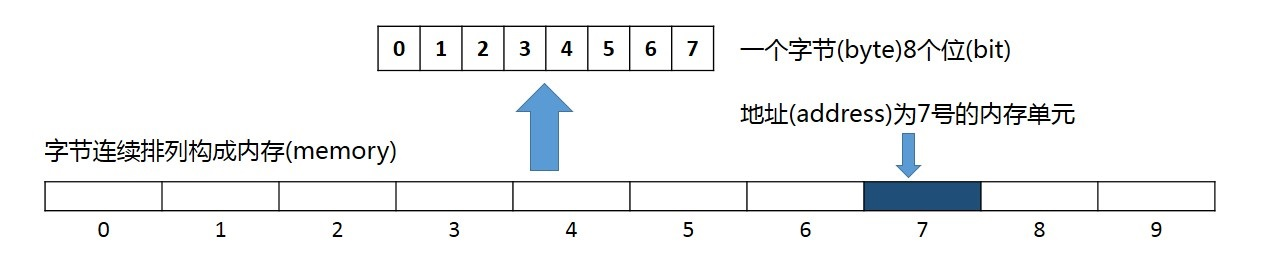
\includegraphics[scale=.5]{../src/memory_01.jpg}
\caption{像一条长龙一样排列的内存}
\label{fig:memory_01}
\end{figure}

\newpage
\subsubsection{寄存器变量}
寄存器是被封装在CPU中间的,不同类型的CPU他的寄存器个数都是不同的。一般来说,32位的机器有8个通用寄存器EAX,EBX,ECX,EDX,EBP,ESP,ESI,EDI,这些不要求大家记住;64 位就更多了,在此不列举了。我在这仅仅告诉大家有这么8 个寄存器,再告诉大家一个基本的常识:CPU读写寄存器的速度比读写内存的要快,而且往往快了很多个数量级。而其他的作用我们在下文中再列举。

\subsection{程序和进程}
这部分首先讲述了如何从C语言变成机器语言,然后展开讨论内存中发生了什么,寄存器中发生了什么,以及他们直接的相互关系。

\subsubsection{内存中的变化}

首先我们来看看C语言是如何变成可执行文件的:

\begin{figure}[bpht]
\centering
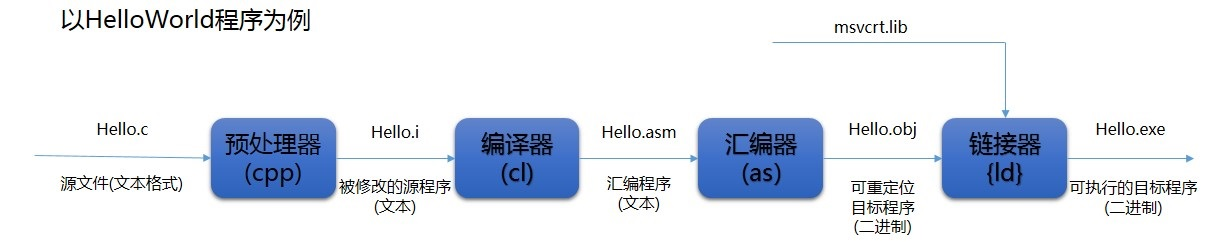
\includegraphics[scale=.5]{../src/cmpSys.jpg}
\caption{编译系统}
\label{fig:cmpsys}
\end{figure}

在标题上大家又看到一个新的术语,\kw{进程(process)},这个还是好理解的。我们写完程序,编译OK了以后,生成\kw{可执行文件(executable file)}\footnote{在Windows系统下是以exe为扩展名的文件,在Linux 下可执行文件一般是没有扩展名的}。如果不运行它,它就静静地躺在磁盘里。如果它动了起来,那他就是进程了。\textbf{注意在下文中,我说到的C语言变量(int, char, double)还包括全局变量之类的,是指我们在写C代码时候定义的变量,而内存变量或寄存器变量是指进程运行过程中的变量是在蹲在内存中还是在寄存器中的变量,千万不要搞混!}

从图  \ref{fig:cmpsys} \footnote{以后若没有特殊情况,文中写到的编译、编译链接就是指图中这么一个完整的过程}中我们可以看到,我们写的C代码,比如 int a = 5; 最后变成了如01010...这种二进制序列东西。好,下面又有写死记硬背的东西了:
\begin{itemize}
	\item 在可执行文件中,不管你是操作(如加法操作a+b)还是数据(a的值是5),通通的是01010...这种二进制序列
	\item 可执行文件不运行,这些0/1序列躺在硬盘里,要运行了,这些序列被拉到内存里面,此时产生了进程
	\item 到了0/1序列被拉到内存中,那么每个内存基本单元字节放8个0/1的序列,也就说每个位只放一个0或者1。
\end{itemize}

读到这您可能会产生疑问,都是0/1构成的序列,计算机如何区分哪些是数据,哪些是操作,又是从哪个地方开始执行程序呢?这个解释起来很麻烦,牵涉到很多东西,但是告诉您:它反正有办法区分,您不要管。这你学了汇编语言之后就知道了。

\textbf{我们可以进行这么一个简单想像:在C代码中我写了个全局变量\footnote{这里为什么要用全局变量,因为我要保证它编译完成之后运行起来一定要在内存中占有内存空间}int a = 5;则a的值是5,用2进制表示是101即可,但是他是个int类型,在x86 模式下占32位,程序在运行时内存要给它一席之地,就得划出四个字节给他,多出来的空位怎么办?当然用0来补充就行了,我们假设我们安排a的首地址编号为38\footnote{一般来说32位机器在内存中安排某个变量的首地址都是4的倍数,也就是二进制最后两位为00},于是乎在“大端模式”(Big Endian)的内存中:}

$$\begin{tabular}{|c|c|c|c|c|}
	\hline
	 & 0000\ 0000 & 0000\ 0000 & 0000\ 0000 & 0000\ 0101 \\
	\hline
	地址编号 & 38 & 39 & 40 & 41 \\
	\hline
\end{tabular}$$

\textbf{在“小端模式”(Little Endian)的内存中:}

$$\begin{tabular}{|c|c|c|c|c|}
	\hline
	 & 0000\ 0000 & 0000\ 0000 & 0000\ 0000 & 0000\ 0101 \\
	\hline
	地址编号 & 41 & 40 & 39 & 38 \\
	\hline
\end{tabular}$$

{\color{red}首先,大小端模式是计算机数据排序的两种方式,您也许听都没有听说过,这没关系,但是要申明一件事,现在的计算机内部几乎都使用小端模式进行排列,网络传输中还使用大端模式,但是小端模式阅读很别扭,希望您能习惯。}

这个想像很重要,我都用黑体加粗了。没明白的再看几遍!而且还有个事要说明一下,刚刚说道要划出32个位给a,细心的读者就会发现,这32个位,正好是从地址为32号的那个字节的第一个位开始安排,那能不能从32号的那个字节的中间位开始依次排好这32个位呢?答案是NO and NEVER,给内存安排东西,先看看图 \ref{fig:memArragment},至少是一整个字节去安排,不会来个第几个字节多少位开始来安排的。

\begin{figure}[bpht]
\centering
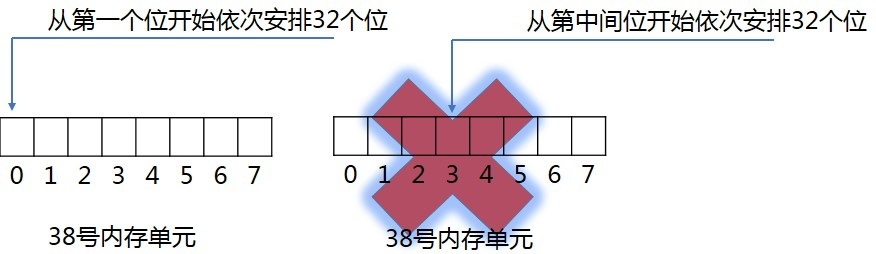
\includegraphics[scale=.5]{../src/memArragment.jpg}
\caption{内存安排}
\label{fig:memArragment}
\end{figure}

看懂了以后,那我现在来问您,第39号地址存放的是什么啊?显然,这个字节存放的是8 个鸭蛋嘛;41号地址呢?答案就是0000\ 0101。而且还要说明一个事,以后写地址编号,我不再使用十进制数来表示了,我以0x 开头的16进制来写,而且地址编号都是由8 位所构成,比如 0x0000 0026 就是刚刚所说的十进制的38号地址。这样以来,我要我们要修改a,在我们C语言里面,你可以这样写,a = 8; 就完事了,到了计算机里面了,a 被安排到了以0x0000 0026开始的4个字节里存放,那么就从这个地址编号开始的4个字节里面塞进去0000 0000 0000 0000 0000 0000 0000 1000,原来的那个二进制的5,自然就被覆盖了。

刚刚我们看到了数据存放的一个模型,再来看那条语句 a = 8; ,他是个操作,是个赋值操作,上面说了不管是数据,还是操作,都有二进制序列构成,所以这个操作的二进制代码是:
$$1100\ 0111\ 0000\ 0101\ \textcolor[rgb]{1.0,0.5,0.5}{0000\ 0000\ 0000\ 0000\ 0000\ 0000\ 0010\ 0110}\ 0000\ 1000$$

显然,计算机会在内存中安排7个字节给这个操作。我们用一个更专业的术语来描述这些由字节构成的操作——\kw{指令(instruction)}。看到这,您有可能猜想,红色的数组,就是那个38,前面的那2个字节表示这条指令的作用是赋值,中间的4个字节表示a所占用的内存的起始地址编号,后面的2个字节用二进制来表示数字8。 呃,这种猜想并不无道理,但实际情况并不是如此简单,往往很复杂,不同的操作,用0/1这种序列来表示长度不一定相同,即使是同样的指令,但是最后的二进制序列长度也不一定相同。上面是7个字节构成一条指令,说不定下一条指令是4个字节或者8个字节。\textbf{程序运行时这些对应指令的二进制序列同样也被拉到了内存当中},您放心,计算机它自然有办法识别每一条指令的长度,我们无须担心,至于为什么,在此不做解释。

\subsubsection{再来看看寄存器}
我上面有个脚注写到了,为保证我编译链接后生成的是内存变量,写的是个全局变量a,如果我是个局部变量a\footnote{如果您不清楚局部变量和全局变量的话,可以查阅相关资料,也可以往后继续读,这并不重要}呢?比如:int i; for(i = 0; i < 100; i++)\{ balabala... \}我们使用这个i,仅仅作为一个计数器,用完了这个for循环,以后就不用了。类似于这种需要空间不是很大,局部性的、用的比较频繁而且一次用完常常就扔掉了的变量,编译完生成可执行文件,在运行的时候往往是寄存器变量。因为上文说道过,对寄存器变量比对内存变量访问读写要快很多。

上面说到了8个寄存器,其实寄存器也有地址,只不过他们的地址编排方法跟内存字节不同,那8个寄存器都有自己的地址编号,例如:0号对应eax,1号对应ebx等等,但是具体对应法则要问CPU生产商。一个内存的地址编号对应一个内存字节,一个内存字节是8 位,换句话说一个内存地址编号对应8个位;而一个寄存器地址编号对应一个寄存器,一个寄存器是32位的,也就说一个寄存器编号对应32位。这点请大家注意。

而读到这可能会有这样一个疑问,我都要写3号地址下的数据,是往寄存器中写,还是往内存中写呢?这个指令中自有办法做出判断,我们无需担心。那我们在C语言中定义的变量,到最后变成了寄存器变量还是内存变量呢?一般来说,C语言全局变量会在内存中固定的划出几个字节给这个变量,至于其他的,跟编译器和编译原理有关,在此不做解释。

总而言之:\textbf{写的程序,不管是数据、对数据进行操作的指令,还是程序控制操作的指令,都是长度不一定相等的二进制的0/1序列,都被拉到了内存中,用一个个字节给他们安排位置,那么这样每一个指令有他的内存起始地址编号,每一个数据也都有他的起始地址编号(内存的、寄存器的都行)}\footnote{当然包括那些个I/O变量之类的,以后下文没有明确指出是寄存器编号地址,指的都是内存编号地址。这句话很重要,希望大家多看几遍记住他}。

我们又来想像一下,请注意,这次的想像与上次毫无关系!程序指令在内存中,一条接着一条被执行。赋值语句如上,那么我们写程序遇到跳转呢?比如if(a>0)\{balabla...\} 这种呢?还记得goto 吗?我们学C语言的时候,老师说到goto,就说他臭名昭著。是的,goto确实破坏了结构化的程序,使代码晦涩难懂,但是想想看,对于if而言,计算机做了个判断a是不是大于0,不是的话就像goto一样跳走,这样做未尝不可呢?

$$\begin{tabular}{cll}
\hline
		& C语言 & 程序指令 \\
\hline
	语法 & goto:loop; & 跳转指令(含地址)\\
	效果 & 跳到loop所在行 & 跳到某个地址开始执行那个地方的指令\\
\hline
\end{tabular}$$\indent {\small NOTE:那个loop是个标签,你也可以改成shit}

图 \ref{fig:ss_01}只是一个想像的模拟场景,里面的地址也是我虚构的,什么大端法小端法问题也没管了,简单到极致了。实际上是很复杂的,我又不说了,o(∩\_∩)o 哈哈~。 函数调用跟这情况有点类似,只不过跳了过去执行完函数就得跳回来,还有函数嵌套了怎么办?这些问题在计算机中通过控制栈帧的方式跳来跳去得以解决,在此不说了。

\begin{figure}[bpht]
\centering
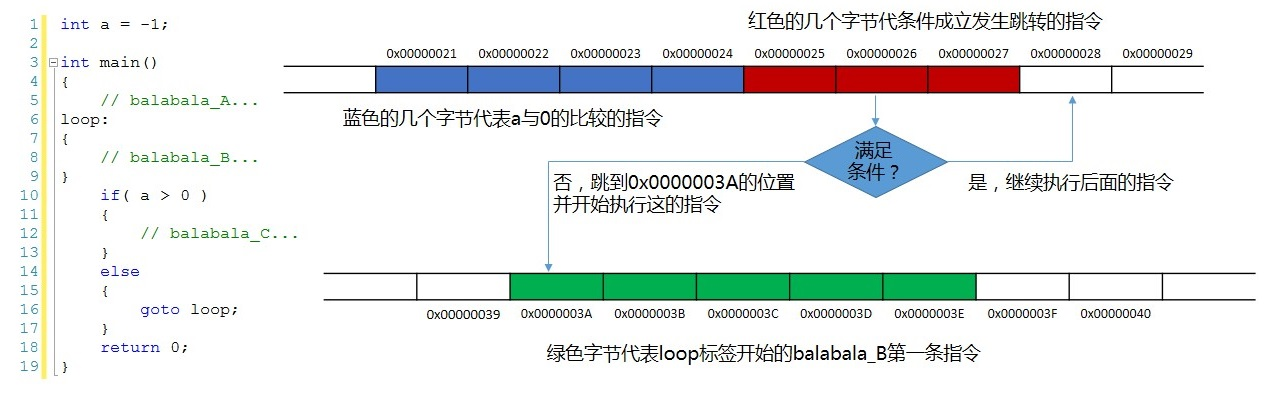
\includegraphics[scale=.5]{../src/ss_01.jpg}
\caption{if举例}
\label{fig:ss_01}
\end{figure}

\subsection{重要的解释}
读到这,如果您还清醒的话,那是最好的,如果您还想到这个问题,那您就NB了:
\begin{center}\textbf{谁负责安排这些地址?}\end{center}

或许您若隐若现的想到了:操作系统搞这事?其实不然,回过头看那张图\ref{fig:cmpsys},图的最右边最后我们看到了\kw{链接器(Linker)}这个我们经常忽视他的东西,却神一般的存在,他把那几个.o文件进行重组,为那些个内存变量安排地址和一条条的指令安排内存空间。这样,我么在C语言写了个全局变量a,也从因此消失不见了,main函数的标志——'m''a''i''n'这几个标识符,也消失了。到了计算机中,执行程序时,自然会有办法找到这个可执行文件中第一条指令所在的地址并开始执行。\textbf{在计算机程序执时行访问一切变量,执行任何一条指令,都是获得这个变量或者指令的确切的首地址,然后进行操作}。

读到这您可能会产生质疑:链接器如何安排地址使得两个程序进程地址不冲突?假如我有两个可执行文件A.exe和B.exe,这两个可执行文件中都写了条对0x0000\ 0026\footnote{还记得这个16进制数的十进制是多少么?}号地址操作的指令,现在同时运行这两个可执行文件,A对该地址编号对应的内存写了个1010 1010,B对该内存地址编号对应的内存写了个0101 0101,那么A读0x0000\ 0026号地址的内容,读出来的就是0101 0101,这样不就乱套了么?错!A读出来的依然是1010\ 1010,B读出来的是0101\ 0101。WHY?这事才真跟操作系统有关,这么跟您说吧:\textbf{由于现代\footnote{如果是早期的16位MS-DOS操作系统,那么访问的确实是物理地址,两个进程读出来的确实都是0101 0101,不过这两条进程不能同时存在,即A在B亡,B在A 亡,而且现在已经绝种了}操作系统使用虚拟地址列表等虚拟化技术,使得每一个进程都有自己独立的虚拟内存地址空间}。也就是说:{\color{red} 在现代操作系统中,进程的内存地址的值是虚拟的,并非是真正的物理内存的地址。}呃,这话有点专业,初学者基本上无法理解,但是您记住有这样的事实存在就行了,至于更深层次的解释,在这不说了。

\subsection{一些补充}
我们给内存编号,下限是0,从0开始编号,那上限呢?

先不讨论上限,我们想想C语言中没有符号的长整型(unsigned long int),他占了4 个字节,也就是32位,所以能表示的数最大是:
$$(1111\ 1111\ 1111\ 1111\ 1111\ 1111\ 1111\ 1111)_2$$
把这个二进制数化成十进制,就是$$1\times 2^0 + 1\times 2^1 + 1\times 2^2 +\dots +1\times 2^{31} = \sum^{31}_{i=0}2^{i} = 2^{32}-1$$
其实怎么推出来的很简单:

{\small $$(1111\ 1111\ 1111\ 1111\ 1111\ 1111\ 1111\ 1111)_2 + 1 = (1\ 0000\ 0000\ 0000\ 0000\ 0000\ 0000\ 0000\ 0000)_2 = 2^{32} $$}

4个字节可以装一个这么大的数,现在我不装这么大,装个小的,比如0000\ 0000\ 0000\ 0000\ 0000\ 0000\ 0010\ 0110如果这个数代表的是一个内存字节的地址编号呢?如果这个无符号的长整型具有这样的功能,我们称这个无符号的长整型为\kw{指针(pointer)}。

其实把上面那个小的代表地址编号的二进制数化成16进制,就是0x0000 0026,没错,就是那个38。那么以后,指针装的地址\footnote{可以这么理解就是4个字节装了个数,这个数代表内存中某个字节的编号}编号我也用0x开头的16进制表示。

这么说一个指针能表示的地址范围就是$\~2^{32}-1$。我们来看看$2^{32}$,如果有$2^{32}$个字节,按照单位换算(依次除以$2^{10}$):
$$2^{32}byte = 2^{22}KB = 2^{12}MB = 2^{2}GB = 4GB $$

那么内存编号的上限是4GB减掉一个字节么\footnote{FUCK!飞哥老喜欢说我:“不强调这一个字节会死啊!”}?说是也不是,因为这牵涉到很多东西,我并不打算做解释。但是有一点希望大家明确,作为一个进程,独享这4GB-1byte\footnote{我就要强调这一个字节}是多么美妙啊!但是也请注意,这么大一块地,也不是说这个进程想在哪搞就在哪搞,你要在哪块地搞,事先必须跟操作系统打招呼,要到操作系统那申请使用,操作系统批准了,你才能用,不然,用指针随便指个地方,然后在上面乱写乱画,操作系统立马把这个进程给咔嚓了。还有指针即使是指向自己的区域也不要乱指,不然你以为自己在自己的进程中的某块内存写东西,实际上是把你的那些控制指令给覆盖了,那就乱套了,异或又被操作系统阻止了,都是有可能的。而且操作系统作为这些进程管理的老大,对于每个进程的内存空间,操作系统都要前面占一些内存,最后面还要抠掉一块约1GB的内存,甚至中间还挖几个墙角,所以你懂的……操作系统这么做,是为了效率\footnote{注意不是“为了部落”}当然只要你写的代码语法、逻辑等都正确,一般不发生诸如雷劈的特殊情况,还是可以很好的使用这些空间。


\newpage
\section{类型和指针}
本部分分成了3个块,分别介绍类型、指针以及类型和指针的关系。最后附加的提一提数组名称的二义性。

\subsection{类型}
说起这个类型,先说说C语言那些基本类型:char、short、int、long、float、double、long long\footnote{其实不止这些,还有什么long double、\_Bool之类的,随着学的越多,慢慢了解吧}之类的,如果您的记忆力好,还发现我漏了个void。在这我不打算一个个详细说,我以int作为例子,其他可以去类推。当然,还会再单独说说void这个家伙。至于signed和unsigned,这个相信学C了基础知识,都很好理解,不说了。

还是来写个全局变量int a;吧,我们知道程序在最后运行时,在内存某个地址开始,往后连续的4个字节放的就是我们现在所写的a的值。要读写的话,就是告诉进程这个首地址,去读写那个地址开始的4个字节就行了\footnote{我有时候也在想为什么不是告诉计算机那4个字节的最后一个字节,然后往上刨4个字节呢?}。

刚刚看到了,对于int这个类型,告诉首地址,计算机就知道,哦,从那开始后面的4个都是要读取或者修改的。如果不是int类型,是char类型的呢?还是好理解,就那一个字节,long和float呢?和int一样也是往后共4个字节,至于double和long long,8个字节。那推广一下,那些个结构体呢?如下图 \ref{fig:struct_01}:

\begin{figure}[bpht]
\centering
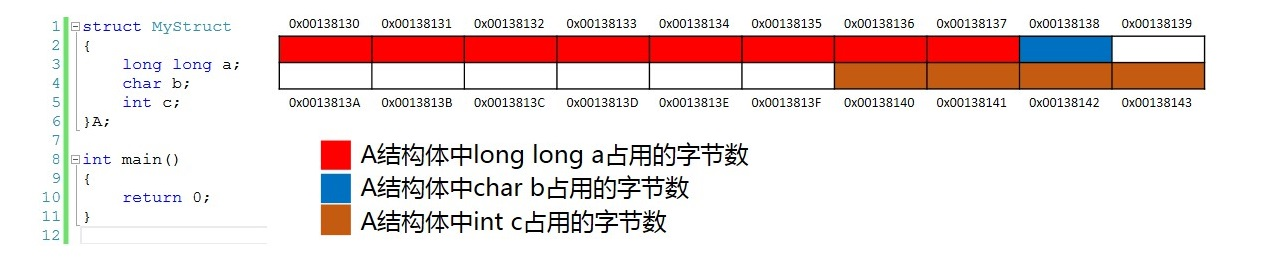
\includegraphics[scale=.5]{../src/struct_01.jpg}
\caption{结构体如何占内存}
\label{fig:struct_01}
\end{figure}

可以从图中看到,这个\kw{结构体(struct)}占用了一块连续的空间,即使是那些空白部分,都是有他的意义的\footnote{因为CPU是按字来抓取东西的,为了提高速度,跟编译时候对齐有关,在此不细说,而且不同编译器空白的区域大小也不一定相同}。我们要修改A中的东西,告诉A的首地址0x0013\ 8130,要修改A中的a,自然,A与a的首地址是同一个,再看看a的类型,哦,long long 的,8个,好那么从0x0013\ 8130开始的8个字节,都是要修改的东西;要修改A中b,首先A的首地址知道了,然后b 相对于A的首地址偏移了8个字节\footnote{如何得到这偏移了8个,这个放心,编译器管,反正最后计算机知道要偏移8个字节},这样,就将A的首地址加8即可得到A中b的首地址0x0013 8138,再看b的类型,一个字节,好,只修改0x0013 8138这一个地址编号里面的东西;最后我们来看看修改A中的c,得到A的首地址,又得到一个偏移量16,而且是int型的,占了4个字节,然后,你懂的……

如果您掌握了结构体,那么我想那些个\kw{枚举(enum)}类型和\kw{联合(union)}类型也是很好理解的。

有些跟编译器和编译原理有关问题我不做说明,前面也提到过,某些变量最后可能变成寄存器变量,根本没有对应的内存空间,对此不做讨论,但是最后确实到了内存空间上面的内存变量,希望大家知道:\textbf{这些变量在C语言代码中用了什么类型,包括他的子类型\footnote{比如结构体类型MyStruct及其子类型long long, char, int},编译器在编译的时候都要做类型检查,如果不匹配,能转换的就转换掉(如int a = 5.8),不能转换的就报错。这样到了计算机执行程序的时候,就知道所有变量的开始地址以及这个变量占了多少个字节,这样计算机才能进行操作。}

再者要重新声明一下,本节从此开始的内容不考虑寄存器变量。

\subsection{指针}

\subsubsection{无类型void}
细心的读者可能发现我漏了个东西——void。void,字面意思是无类型,更准确的说法是现在确定不了的类型。你写个void a;看看,编译器会报错,因为不管最后这个a成为了内存变量还是其他的什么变量,你能告诉我有多少个位么?因为C语言就没规定void类型是多少位,而且你也不能去违规强行定义void有多少位。

但是我们写了个全局void *p;却又对了。这是为何?我们先放下这个问题,来回想下,我们说在内存中划4个字节,也就是32位,里面放了一个二进制数,这个二进制数又代表了另一个地址编号,如图 \ref{fig:pointer_01}。

\begin{figure}[H]
\centering
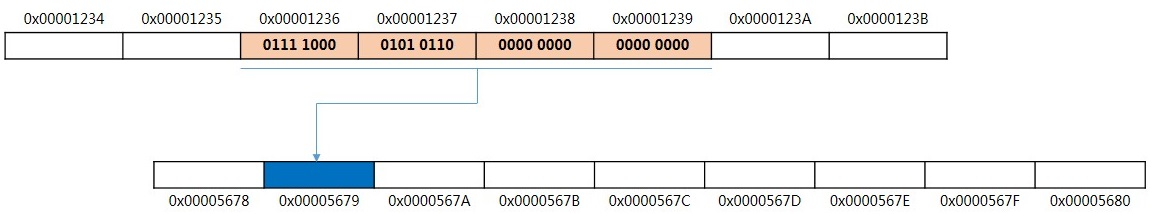
\includegraphics[scale=.5]{../src/pointer_01.jpg}
\caption{指向另一块地址的指针}
\label{fig:pointer_01}
\end{figure}

如果我说0x0000 1236开始的这4个字节\footnote{当然也可以被装到一个寄存器中}正好是p的内容呢?,那么p指向了另一个地址编号为0x0000 5679的内存单元,而地址编号0x0000 5679可能就是一个char类型的变量所在位置,也可能是跟后面三个字节共同组成一个4个字节的int型,或者是跟7个字节组成的long long型,或者是后面跟3个字节又组成另外一个指针,指向另外一个地址,甚至是后面跟了几个字节,组成一条指令也说不定,这跟图 \ref{fig:ss_01}类似。虽然机器不知道指过去的是变量还是指令,又是什么样类型的变量,什么样的操作指令,的但不管如何,这个p指向了一个东西的首地址。

\subsubsection{到底指向什么}
但是,某个东西到底是什么东西?这是您的问题,更是编译器发出的问题。想像一下您就是编译器,我写了int *p;您知道,要在最后生成的可执行代码中告诉机器从某个字节开始抓4个字节进行处理,如果我写了个long long* p;您知道要抓8个字节处理,但是现在是个void *p;您当然不知道要从那个地址开始抓多少个字节处理。由于不知道,很显然,报错!

难道我只能写个void *p;做样子,而不能用么?这就没实际意义了呀!不是的,void*类型实际上是很有用的东西,C语言提供了一个很灵活的语法——\kw{类型转换(type conversion)}。现在我这么一转(int*)p;您作为编译器就清楚了,就按照int *p;的方法处理,即抓4个字节即可。当然,想转成(long long *)p;也行,虽然这个很有用,而且编译器检测语法没有问题,但是,不会用的话到最后执行发生了逻辑上的错误,目测操作系统会一巴掌拍死\footnote{可见这货是把双刃剑}。

\subsection{小总结}
通过以上的探索,我们来总结一下:
\begin{itemize}
	\item 我们写程序时无法获得变量在运行时的内存地址,但是我们知道这个地址可被装进了一根指针。
	\item 指针可分为两部分:值和类型。
	\item 指针的值仅仅只是装了某个东西的首地址的32位无符号整型二进制数\footnote{当然可以化成十进制和16进制,其实我使用16进制表示地址也是习惯上大家都这么用,这样转化不仅方便,而且不用写的像裹脚布一样又长又臭,阅读上也比二进制方便}而已,没有别的。
	\item 机器是不知道指针的类型,执行的时候机器只知道从那个地址开始抓多少个字节。
	\item 而编译器必须要知道这根指针的类型才能生成可执行代码,告诉机器执行时要抓几个字节操作。
	\item 指针指过去的类型可以是C语言规定的基本类型、自定义类型或者是指令。
\end{itemize}

\subsection{数组}
终于要说说数组了,还是老规矩,先写个全局变量int a[100];这样一个程序编译完运行时,会在内存中划400个连续的字节放这个数组,要使用第i$(0\leqslant i \leqslant 99)$个元素,那么告诉a 的首地址,然后算偏移量$a+i\times 4$即可找到第i个元素的首地址,然后抓取这个地址开始的4个字节进行处理就OK了。

请注意这个不起眼的东西$a+i\times 4$,算偏移量的时候,我直接这么写了,难道a是个地址?没错,对于\kw{数组而言,数组名既可以是这个数组的标识符,又可以是这个数组的首地址!我们可以把数组名当指针一样去用}\footnote{请注意这句话的用词:既可以,也可以,这就意味着有时候不完全等价,这个在下文还会提到;而且如果您非常了解C语言的extern关键字,也能知道其中区别,而现在,你就把他们当成等价的就行了},我们对a分别进行直接输出、解地址(*a)输出、取地址(\&a)输出,用printf查看输出效果,如图 \ref{fig:arryadd_01}:

\begin{figure}[H]
\centering
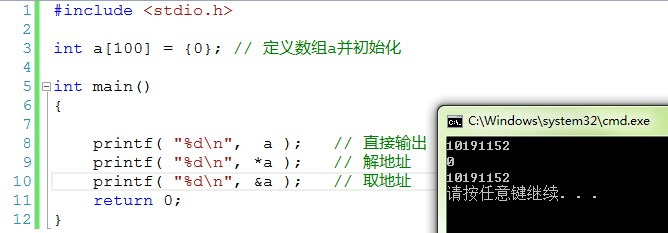
\includegraphics[scale=.5]{../src/arryadd_01.jpg}
\caption{数组名的二义性}
\label{fig:arryadd_01}
\end{figure}

可以看到,直接输出,a化身成了指针,就相当于输出指针中的内容,就是一个地址的数字编号;解地址,跟输出a[0]\footnote{其实[]这个东西,就是为了方便*(p+i)的,p 为首地址,i为往后地址偏移量,*号就是根据p的数据类型,操作相应字节数}一样;而取地址时,a就成了普通变量名,虽然代表了广大的400个字节\footnote{你可以这样认为罢了},但是首地址只有一个,便被取出来输出了。

\newpage
\section{数据类型和指针}
上一节中只是初步说明了指针和类型的关系,为大家建立了一个初步的概念,而这一节的内容主要是起到承上启下连接的作用,补充上一节的知识,为下一节做铺垫。所以在本节,首先我们会深入探讨子类型,然后说明C语言在定义和使用指针时是如何受限于类型。

不过在正式将之前,我们还是理清楚一个概念,我们在定义某个东西的时候,“*”号代表是个指针,至于什么类型,会在“*”号前面说明,如果不知道,就写个*p就行了\footnote{如果您认为void *p是无类型,那就错了,我们认为void也是一种类型,名叫空类型,不确定不等于没有,希望您认真体会};而使用的时候“*”号是根据地址去抓相关内容,抓多少就跟前面的类型说明有关。定义声明的*号与使用时的*是不同的,这点希望您必须明确。

\subsection{类型和子类型}
在上一节的那个小总结中我们可以知道,实际上到了最后的代码中,机器这货只知道从哪个地方开始抓几个字节罢了,并不牵涉到类型的事。理论上我们写个int *p;最后让p去指向一条执行指令也是可以的。但是别忘了,编译器不是那么好糊弄的,编译器要知道类型,你明明写的时候写了个int类型的,然后让p去指向个指令的内存单元,别说编译器不帮忙进行类型转换,就是我们自己也不知道如何转换,所以肯定不让你编译通过。而且不仅如此,\textbf{编译器在编译的时候,不仅会做类型的检查,还会检查他的子类型}。

\subsubsection{深入理解子类型}
何为子类型?还记得我们那个结构体么?一个MyStruct类型下面有三种不同的子类型:long long、char 和 int,这算一种最普通的情况了。但是从此开始,一切不再那么平凡了。

首先我们现在来玩些高端霸气上档次的文字游戏吧。从最简单的开始:定义一个指向整型的指针的指针。好好好,我们先断个句:定义一个/指向整型的指针/的指针。如果您分得清主谓宾等句子成分而且英语水平不是很搓的话,把这句话翻译成英语是最好理解不过的了:Define a pointer which points to an integer。那么我们这么理解:首先最外层的要求是要我们\textcolor[rgb]{0.5,.0,.0}{定义一个指针},好吧,写个*p 就行了;对于次外层(或者说是第二层)而言,它要求是个\textcolor[rgb]{0.5,.0,.0}{指向整型的指针}。

\begin{figure}[H]
\centering
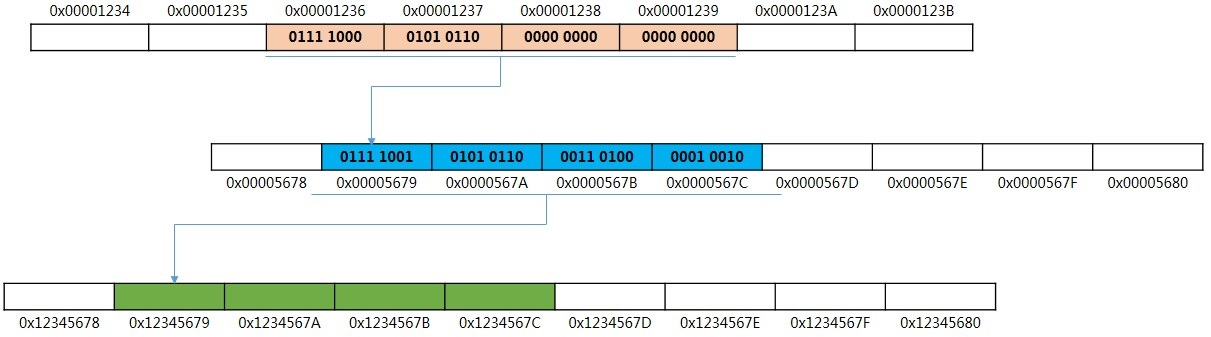
\includegraphics[scale=.5]{../src/sedpointer.jpg}
\caption{指向指针的指针}
\label{fig:sedpointer}
\end{figure}

我们来回顾一下,要写个指向整型的指针,我们这么写int *t就行了;我们把这两句深红色的话组装一下,就形成了我们最开始那句很拗口的“一个指向整型的指针的指针”,如果我们把*p和int *t;也组装一下,用*p 整体代替t,就形成了int**p了,这正是这句拗口的话的含义。没错**p就是我们通常所谓的\kw{二级指针}\footnote{二级指针这种叫法也只有在中国的书籍中这么叫,一般国外都叫Pointer to a pointer}。如果写个全局变量int **p;最后在计算机里面目测效果如图 \ref{fig:sedpointer}最里面,指向了一个绿色的int数。

\subsubsection{编译器检查}
但是在这需要再次跟您强调一点,这个类型是编译器做检测用的,在机器内执行的时候是只知道从哪开始抓几个字节。类似上面那个文字游戏,对于编译器这个文字控,不仅要检查你这个最外层的类型符不符合,而且第二层,甚至是第三层第四层都有可以能。最简单的例子:定义int **********p;那现在我们有个整型变量int a;,如果要把a的地址赋给p,那么就得p = \&\&\&\&\&\&\&\&\&\& a;

也许细心的读者会发现,我把最外层的那个指针(图 \ref{fig:sedpointer}中浅咖啡色)名字叫p,那第二层的那个指针(图 \ref{fig:sedpointer}中浅蓝色)的指针叫什么名字呢?如果你想说无名,那就错了,应该说名称不固定。什么意思呢?假设我这有两根指针,分别是int *a; int *b;,这个二级指针p既可以指向a,又可以指向b,到底指向哪一个,根据具体情况而定。而且就类比*a这个指针,现在有c和d 两个整型变量,到底指向哪一个,也说不定\footnote{而且这些32位的东西,有些还放到寄存器里面,情况更为复杂}。但是总之,指向的类型及其子类型甚至是孙子、曾孙类型都要要匹配才对。

\begin{figure}[H]
\centering
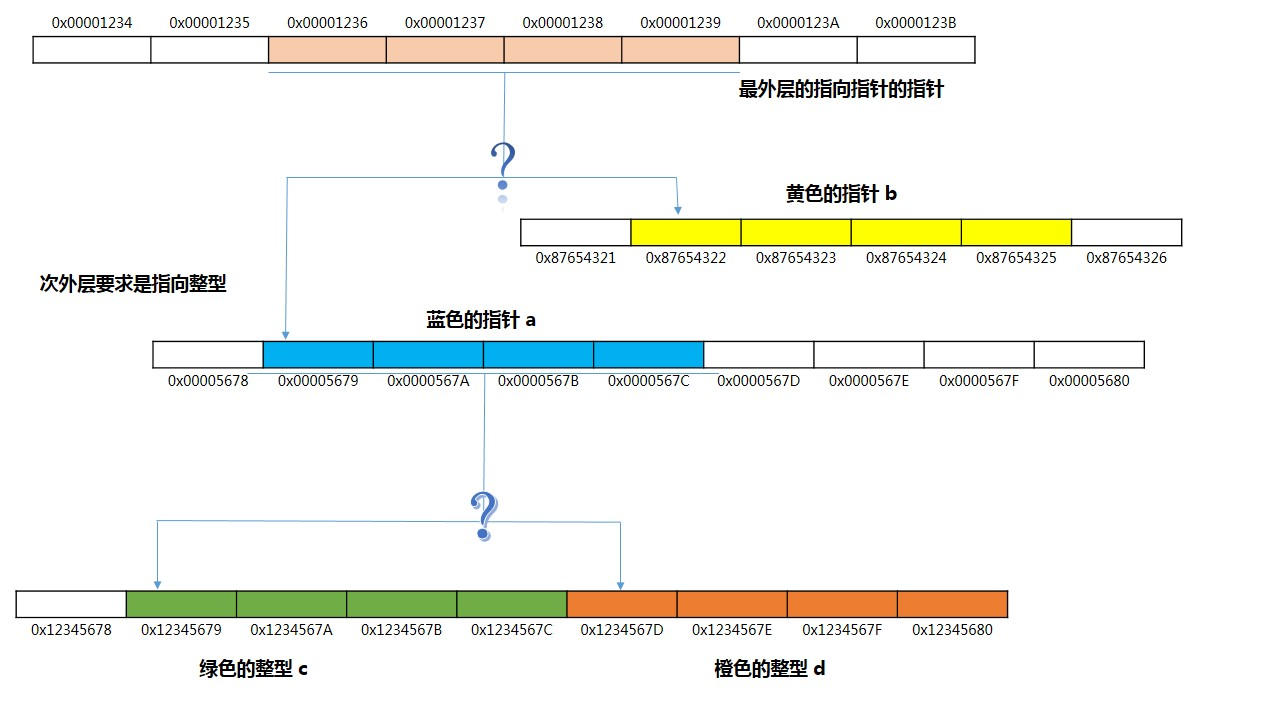
\includegraphics[scale=.5]{../src/uncertain.jpg}
\caption{不确定的指向}
\label{fig:uncertain}
\end{figure}

C语言正是有了这种不确定的指向,才使得整个编程更有弹性,更灵活。但是这是把双刃剑,用得好,写出来的的代码非常优美简洁、可读性强而且效率高,用的不好,又烂又臭,而且编译器只检查类型匹配不匹配,不检查越界之类的逻辑错误,这种烂代码运行时常常因为逻辑错误而挂掉\footnote{我们用一个更专业的术语——\kw{运行时错误(runtime error)}来形容这种情况}。

\subsection{一点小区别}\label{sec:diff}
刚刚在前文中所看到的那个十层*,一般人不会写出那样的代码。但是,现在我要求写:定义一个指针,指针指向一个整型数组。

别急,我们按部就班,一层一层来,首先要一个指针,好吧,*p,就你了;指针指向一个数组,我们想想,平时要写个数组是不是写个a[],整型的就是int a[];即可,而现在要这个指针指向这个数组,那么我们把*p 和int a[]组装一下,名字只要外层的,用*p 整体代替a,是不是就形成了int (*p)[];\footnote{注意不是int *p[],这是为了避免歧义,如果写成了int *p[],编译器会理解成定义一个数组p,数组每个元素都是一个指向整型的指针,即每个元素是int *类型}

好,如果您认为int (*p)[]是正确答案,那么恭喜您,答错了~正确答案是int* p;WHAT?我没有逗您,而且赋值的时候,要明确把数组(如int a[8])的数组名就是地址,不能显式调用\&取地址,即必须写成p = a;写成p = \&a;就是错的。

我们在前面就说过了,一个数组的数组名,既可以是个名称,又可以是个指针,装的就是数组的首地址。而我故意写了句话,迷惑了您。先别生气,想请问下,那个错误答案int (*p)[]是什么意思呢?答案是这样的:定义一个指针,指针里面的元素都是一个整型数组,但是每个数组的长度必须要标明,就是说那个中括号[]里面必须要确定多少个元素。看下这个图 \ref{fig:diff_01},想想为什么。

\begin{figure}[bpht]
\centering
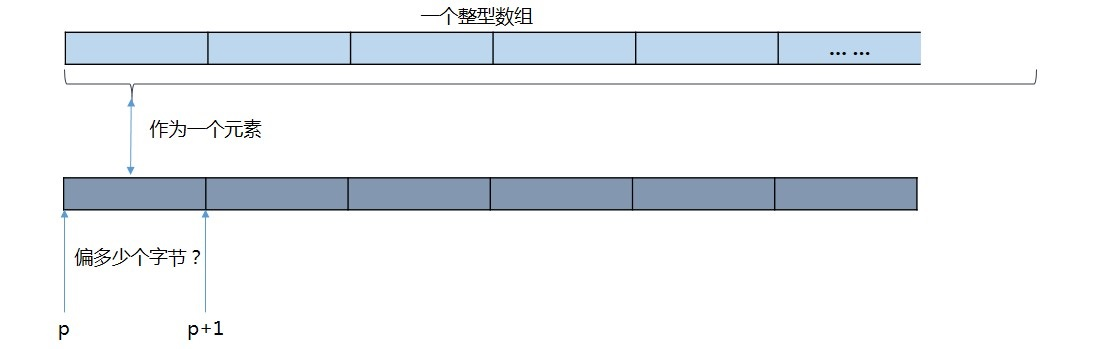
\includegraphics[scale=.5]{../src/diff_01.jpg}
\caption{如何偏移}
\label{fig:diff_01}
\end{figure}

如图所示,我们把一个指针数组看成一个整体,作为一个另一个数组的一个元素,现在用p指向这个数组,如果不告诉我这个整型数组具体有多少个元素,那么我计算p+1的时候,到底要偏几个字节呢?这就是为什么要确定这个[]中的数字的原因了。

\subsection{数组小问题}

\subsubsection{越界问题}
刚刚这个int (*p)[]牵涉到二维数组,我们暂时不管,但是我们回过头来看int *p;,然后有个整型数组b,我们把这个数组的首地址赋给p,即p = b;然后我们可以用p[i]或*(p+i) 来调用数组b中的第i+1个元素\footnote{别忘了数组下标从0开始,b[0]是第一个元素哦}。现在我们现在只知道有个这么个数组b,却不知道b有多少个元素,万一b中只有8个元素,我写了个p[10],就不对了啊!是的,这发生了严重的逻辑错误,请一定注意:\textbf{编译器他只负责类型对不对,不会去检查越界这种问题},这会使得程序跑的时候挂掉。不仅如此,你写个p[-1]也是可以的。

\subsubsection{定义数组名}
在定义的时候,虽然有时候写type\_name *p和type\_name p[]是等价的,但是更多情况是不等价的,使用sizeof运算符或者牵涉到多维数组的时候,问题就明显了,在此我并不打算深入探讨,下文中若出现等价情况,我会写个脚注标明的。但是以后看到我写了个定义一个数组什么的,凡是没告诉您有具体多少个元素,则写成type\_name* p形式,如果明确了数组中的元素,则使用type\_name p[] 这种形式更为合理,反之亦然。

\subsubsection{丢失问题}
还有一个小问题,我们如果定义一个全局变量char *p = "balabala";和定义一个char p[] = "balabala";是有很大的区别的,前者的p,现在指向的是一个字符串“balabala”的首地址,但是这个p还可以指向其他的字符串的首地址,也就是说,写个p=a;(a 为另一个字符串)是合法的;而后者那样去定义的时候,p就只能是字符串“balabala”;的首地址,不能改变,也就是说再写个p = a;是违法的。

我们来谈谈char *p = "balabala";这个定义,请看下面代码:

\begin{lstlisting}
char *p = "balabala";
char a[] = "lady_gaga";

int main()
{
	p = a;
	// other body...
	return 0;
}
\end{lstlisting}

现在请问,我如何找回这个“balabala”的首地址呢?答案是找不回的,而且操作系统却认为这块内存任然属于你这个进程,又不允许别人来占用,哪怕就是再申请内存,操作系统也不会再分配利用这块内存。总而言之这块内存占了地方我们找不到,没法用,这便是传说中的典型的\kw{内存泄漏(memory leak)}。但是如果我么写成char p[]=“balabala”;时p是固定的,没法改了,这个问题也就不存在了。

虽然有时候我们不知道这个p到底是数组名还是一个指针,能否对其赋值,但是我们知道,都可以使用*(p+i)或者p[i]去获取元素,用直接赋值q = p的形式去赋值就行了。

\newpage
\section{函数类型和指针}
前面我罗里吧嗦写了那么多,相信看官老爷您看得有点不耐烦了,但实际情况是:重头戏才刚刚要开始。

而在重头戏开始之前,我还是会剖析函数到底是个什么玩意,把他与我们上面所讲的指针、类型联系起来,从而形成一个整体观。

\subsection{函数}
说起函数,我们还是先来看看函数的构成吧:

\begin{lstlisting}
return_type function_name( par_type par_name ... )
{
	// function_body...
	// balabala...
}
\end{lstlisting}

函数大体都长这个样,首先有几个常识性的东西我在此列举:

\begin{itemize}
	\item 在C代码中的函数,经过编译完之后,在机器代码中以一条条的指令呈现出来
	\item 函数定义的时候,函数名既代表函数的名称,又代表函数的第一条指令的首地址地址编号
	\item 函数的类型可分两块,参数类型和返回值类型
	\item 说函数类型相同,则参数类型和返回值类型都相同,还包括参数个数和参数类型顺序也相同
\end{itemize}

还记的我曾经在本文最开始的时候说那个指令是什么吗?无非也是几块连续的字节构成的嘛。几块字节,既能构成数据,也能构成指令。在C代码中定义变量,最后在字节便构成了数据,而定义\footnote{注意,这是函数定义,跟函数声明不同,在本文不细说,但是这个内容很重要,望您查阅相关资料}了函数,则变成了指令。既然是指令,肯定有第一条呗,我们调用某个函数,那么就是从这个函数的第一条指令执行,怎么返回,我这就不说了。而且函数名代表的就是第一条指令的首地址\footnote{这话说的我自己都感到很别扭},既然是个地址,我们可以当指针一样去处理,比如我们定义一个函数int fun(double a );,那么我们在调用的时候可以写成fun(a);也可以写成(*fun)(a);,这跟数组名的二义性是类似的。

函数的类型分成了参数类型和返回值类型。这个参数类型不仅要求参数的类型相同,个数相同,而且排列顺序也相同,比如int fun(int, char)和int fuck(char, int)这两个函数的参数类型就不同了,虽然都是1个int一个char,但是摆放位置不对应。返回值类型可以是我们的基本变量类型、自定义的诸如struct、enum等类型,也可以是指针,比如返回int*型的函数int* fun();。

\subsection{用指针指向函数}
我们首先来回顾一下,我们要定义一根指针,写个*p就好了,要这根指针指向一个int 型,则在前面加上一个int,即组成int* p就行了。而函数了?

这样,先假设我们已经存在这样一个函数int fun(int a,char b)。老规矩,首先最高层的要求是要定义一根指针——*p,然后,要指向这个函数了,我们任然采取组合替代的方法,保留最高层的名字,用*p去整体代替fun,那么就形成了我们最终想要的\kw{函数指针(pointer to the function)}:
\begin{center}
\textbf{int (*p) (int a, char b );}
\end{center}

您可能想组合的时候能把(*p)的括号去掉吗?不能!去掉的话会产生歧义,一旦去掉,变成了\textcolor[rgb]{0.7,.0,.0}{int *}p (int a, char b),编译器认为int*是一个整体,认为这是个返回值为整型指针的函数,而并不是一根指针去指向一个函数。

\textbf{定义函数指针的时候,由于函数的类型包括了返回值类型和参数类型,两个类型,所以,把返回值类型放左边,中间用(*p)作为指针标志,把参数类型用括号括起来放到右边,形成了 \framebox(20,8){}(*p)( \framebox(30,8){} )的样式。希望大家尽早熟悉}。

好了,现在这个p指向了fun这个函数,调用的时候,我们可以像普通函数写法一样写成p(c,d);,也可以写成(*p)(c,d);。p这个指针不仅能指向fun这一个函数,还能指向其他的函数,只要其他的函数符合一个条件:返回值类型必须是int,参数类型从左到右依次为int和char。那您或许会问,参数类型依次为int、char,那参数名要符合么?答案是不需要的。还记得我么曾经说过的,名称到机器里面是没有的,所以编译器只检查类型,而忽视参数名。既然忽视参数名,那参数名写了也白写吗?是的,所以,经常在定义一个函数指针的时候,常常不写他的参数名称,所以更常见的是int (*p)(int,char)这种形式。

好了,现在我们定义了int (*p)(int,char)这个函数指针,我们来做几个题吧,对于下列函数,哪些是可以用p=fun(或p=\&a)表示:
\begin{itemize}
	\item int *fun( int a, char c );
	\item int fun( int a, int c );
	\item char fun( int a, char c );
	\item int fun(int,char);
\end{itemize}

第一个,肯定不行,返回值要int,不要int*;第二个不行,参数不对;第三个也不行,返回值错了;第四个,是正确的。虽然这个函数只有参数名,没有参数,但是他符合我们的赋值条件。而且我们在定义函数指针的时候,更强调的是指针的名称,而不是参数的名称,所以,写成int fun(int,char);是更常见的形式。

我们写两个指针,int *p;和int *q; 可以相互赋值,即p=q;,函数指针归根结底不过也是个指针罢了也支持这种相互赋值,比如int (*p)(int,char)和int (*q)(int a,char b)也能相互赋值,比如p=q;

\subsection{可怕的排列组合}
做题吧,请按要求写出下列内容;

\begin{itemize}
	\item 定义一个指针,指向一个函数,函数的参数一个为int,一个为char,函数的返回值为void
	\item 定义一个指针,指向一个函数,函数的参数为一个指向整型数组指针,函数的返回值为int
	\item 定义一个指针,指向一个函数,函数的参数一个为int,一个为char,函数的返回值为一个指向数组的指针,数组的元素全部是指向整型的指针
	\item 定义一个指针,指向一个函数,函数的参数一个为int,一个为char,函数的返回值为一个指向函数的指针,该函数的的参数一个为int,一个为char,返回值为int
	\item 定义一个指针,指向一个函数,函数的返回值为int,参数是一个double 和一个指针,指向一个函数,函数的参数为long long,返回值为整型指针。
\end{itemize}

第一个,还是中规中矩,我直接写了:void (*p)(int, char);。

第二个,首先最外层,要求是个指针——*p,指向函数,不用说了,就是这种形式: \framebox(20,8){}(*p)( \framebox(30,8){} ),参数为一个指向整型数组的指针,就是int *q\footnote{在明确数组元素个数的情况下,可以写成int q[]},嵌进去,就是\framebox(20,8){}(*p)( int *q ),最后,返回值是int,即:int (*p)(int *q)

第三个,首先是一个函数指针,\framebox(20,8){}(*p)(int,char),函数的返回值是\textcolor[rgb]{.0,.5,.0}{一根指针,指针指向一个数组,数组元素都是整型指针},这段绿色的话可以用int* *q\footnote{同样,若明确数组元素个数,可以用q[] 代替}来表示,最后,将q用(*p)(int,char)整体代替,便得到最终答案:int* *(*p)(int, char);

其实函数指针这种东西,还包括子类型的描述,用文言文句式(尤其是定于从句)在好不过了,现在语法不是那么好描述,或者我们干脆用英语来描述,那么第三句就是:Define a \uline{pointer to a function} whose \uline{parameter-types are int and char} and that \uline{returns a pointer to an array} whose \uline{elements are a pointer to an integer}。这样一来,是不是清晰多了?

后面两个,我给出英文翻译和图\ref{fig:qustion_01},您先别看后面的答案,自己试试。

\begin{itemize}
	\item 4:Define a \uline{pointer to a function} whose \uline{parameter-types are int and char} and that \uline{returns a pointer to a function} whose \uline{parameter-types are int and char and that returns an integer}.
	\item 5:Define a \uline{pointer to a function} that returns an integer and which owns two parameters, where the first is the double, and the second is a function pointer that \uline{points to a function} whose \uline{parameter-types is long long} and that returns a \uline{pointer which points to an integer}.
\end{itemize}

\begin{figure}[H]
\centering
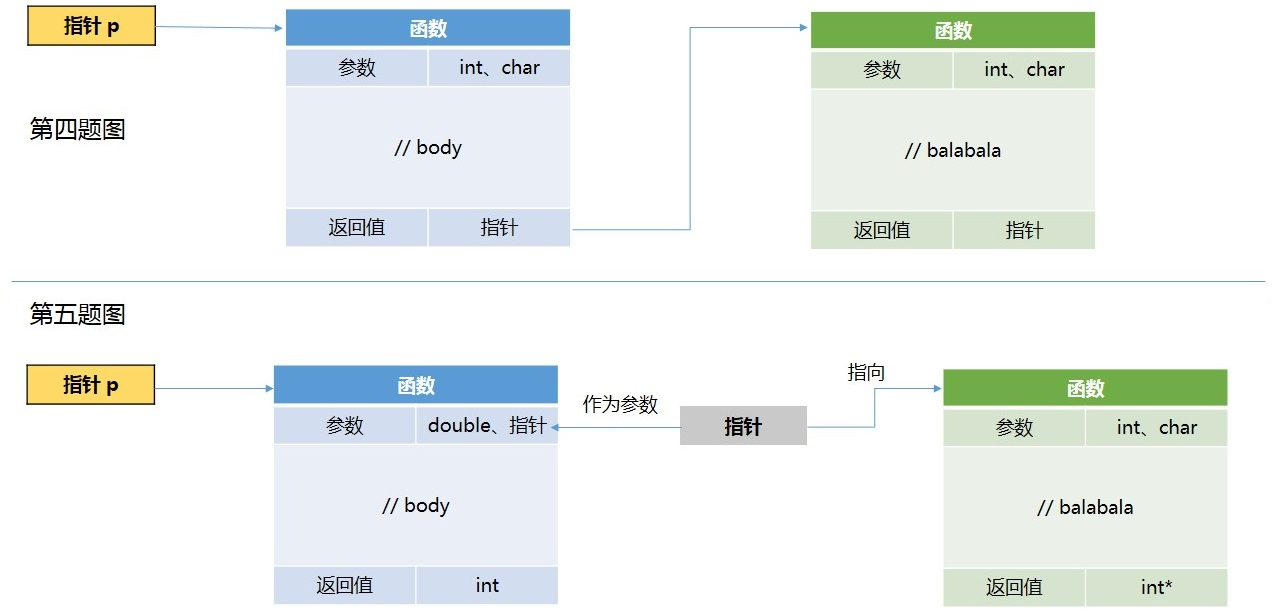
\includegraphics[scale=.5]{../src/qustion_01.jpg}
\caption{题图}
\label{fig:qustion_01}
\end{figure}

答案:见脚注\footnote{4:int (*(*p)(int,char))(int,char) \\ 5:int (*p)(double,int* (*fun)(long long));}

\subsection{压轴大题}
好了,如果你能正确做出上面这些题目,逆向来相信这个也难不倒你:

%int* (*(*(*p)(int**,int*))(double,char))(float,long long*);
\begin{center}
int* (*(*(*p)(int**,int*))(double,char))(float,long long*);
\end{center}

哈哈,被坑了吧,我不用语言去分析这个了,直接上图:

\begin{figure}[H]
\centering
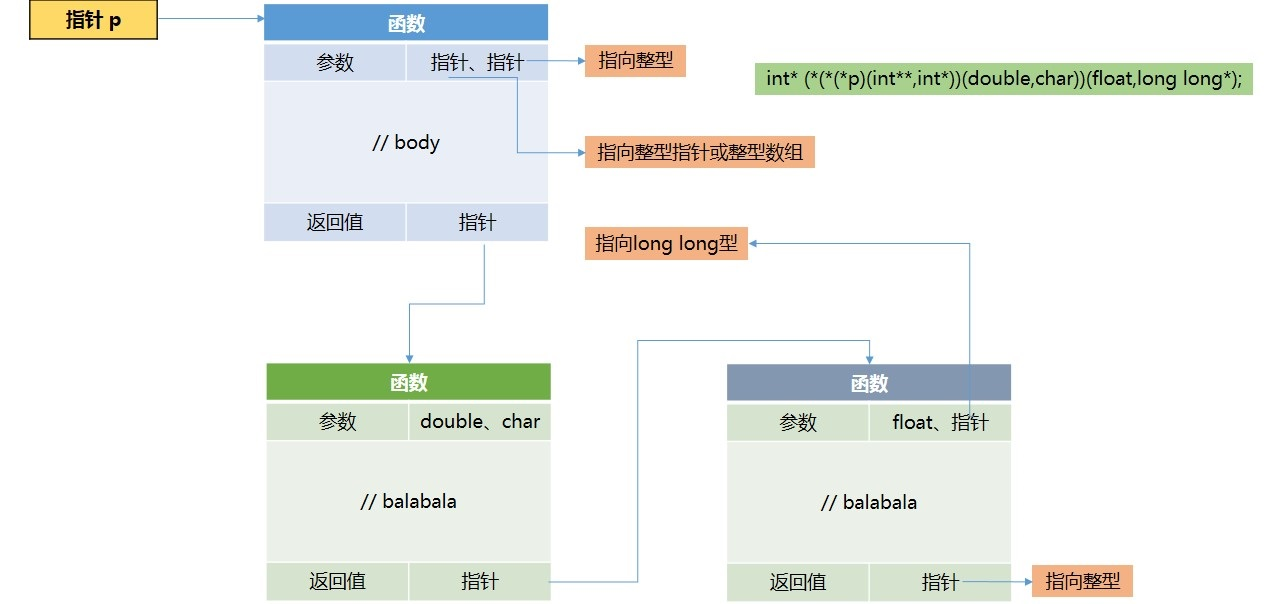
\includegraphics[scale=.5]{../src/cmpfunpt.jpg}
\caption{丧心病狂的函数指针}
\label{fig:cmpfunpt}
\end{figure}

其实这个是我故意搞的,实际上在写代码的时候,不会去这样写,即使某些表达式最终展开了是这个形式,也是通过typedef这个关键字一层一层的架设起来的,但是那些简单的函数指针(如int (*p)(double, int) ) 知道是非常必要的。而在一下一节,我们的最后任务,即使讨论typedef这个关键字。我将会一步一步typedef,把这个常常长的函数指针用typedef的形式展现出来,层次分明。

\newpage
\section{关键字typedef}
在开始之前,我希望您能从上一部分最后的那个东西中缓过神来,然后再阅读本节内容。typedef这个关键字用的作用范围很广,尤其是一些工业级的代码,那真的是typedef和\kw{宏(macro)}满天飞的。使用typedef 不仅在写代码的时候可以变得更灵活,而且对于阅读代码的人来说,typedef使得代码更容易理解。

在本部分内容中,我并不想多分析typedef如何如何使用,只是告诉您typedef的一个最基本的功能——\textbf{取别名的作用}。首先我们会谈到一般变量如何取别名,然后,谈谈函数指针如何取别名,最后我们将上一部分最后那个长长的函数指针一步一步typedef 架设起来。

\subsection{变量取别名}

\subsubsection{一般取别名}
我们从最简单的开始讨论,请看下面这行:
\begin{center}
{\color{blue}typedef} {\color{violet}unsigned long long} u64;
\end{center}
这行代码,就是为unsigned long long 取了个叫u64的别名,以后我们要定义64位无符号整型,觉得写unsigned long long a; 太麻烦,直接就可以写成u64 a;了,这样可以省敲键盘了。

好,我们再来取个别名:{\color{blue}typedef} {\color{violet}int*} LP;\\
那么请问,我现在写了个LP *p;这个p是个什么?如果您回答到是个整型指针,那就错了,想想LP是什么,是{\color{violet}int*},那现在把{\color{violet}int*}代替掉LP *p中的LP,得到的是{\color{violet}int*} *p;看清楚了没,是个指向指针的指针,也就是常说的二级指针。这点对于初学者很容易犯错,所以希望您能细心一点。

\subsubsection{结构体取别名}
在说结构体取别名之前,让我们来重温一下一般结构体吧,在全局范围内写个:
\begin{lstlisting}
struct MyStruct
{
	int a;
	float b;
}MS,*MSP;
\end{lstlisting}

在这里,没用typedef这个关键字,这就意味着编译器会实实在在产生一个8字节变量MS 和一个名为MSP的指针,指向struct MyStruct类型。好,我们现在加上typedef:
\begin{lstlisting}
typedef struct MyStruct
{
	int a;
	float b;
}MS,*MSP;
\end{lstlisting}

这个时候,编译不会产生一个变量或指针,编译器会理解成下面这两段代码:

\begin{lstlisting}
struct MyStruct
{
	int a;
	float b;
};
typedef struct MyStruct MS;
typedef struct MyStruct* MSP;
\end{lstlisting}

那么我们以后定义这种结构体变量,就不用写成struct MyStruct a;而直接可以写成MS a;,如果要定义一个指针,用MSP p即可,注意,千万不要写成MSP *p;,请记得上面说的那个二级指针!

其实,我们可以去掉MyStruct,即:
\begin{lstlisting}
typedef struct
{
	int a;
	float b;
}MS,*MSP;
\end{lstlisting}

这样,妈妈再也不用为我取名而发愁了~

\subsubsection{数组指针取别名}

还记得这个东西么:int *p;

如果在全局环境中写了这个东西,编译器会分配4个字节,产生一个指向整型数组的指针p,如果我们还要定义三个这样的指针,那么就要写:
\begin{lstlisting}
int *p1;
int *p2;
int *p3;
\end{lstlisting}

但是现在我们加上typedef:
\begin{center}
{\color{blue}typedef} {\color{violet}int* p};
\end{center}

此时,编译器不会产生一个指针,会认为p是一个类型代表。可以将上面3个指针p1、p2、p3写成:

\begin{lstlisting}
typedef int* p;
p p1;
p p2;
p p3;
\end{lstlisting}

如果您和我一样懒,可以直接写成:
\begin{lstlisting}
typedef int* p;
p p1, p2, p3;
\end{lstlisting}

是不是少敲了很多次键盘?

那现在请问可以写成{\color{blue}typedef} {\color{violet}int p[]};吗?答案是不可以!这个跟第\ref{sec:diff}节类似,也牵涉到二维数组,故不说了。

\subsection{函数指针取别名}
好了,如果您看懂了对数组指针取别名,我相信您对函数指针取别名也是很好理解的。比如:
\begin{center}
{\color{blue}typedef} {\color{violet}int (*pfun)(int, char)};
\end{center}

这样,下面这段代码中,第一行和最后两行完全等价:

\begin{lstlisting}
typedef int (*pfun)(int, char);

int (*p)(int, char);
pfun p;
\end{lstlisting}

好了,还记得开篇申明中的{\color{blue}typedef} {\color{violet}int* }{\color{black}(*func)}{\color{violet}(int,double)};吗?现在您明白了吗?

\subsection{做些习题}
好了,到最后,我们还是来做些习题吧,请看如下代码:

%int* (*(*(*p)(int**,int*))(double,char))(float,long long*)
\begin{lstlisting}
typedef int* (*fun)(float, long long*);
typedef fun (*foo)(double,char);
typedef foo (*p)(int**, int*);

p pointer;
\end{lstlisting}

这段代码从后面往回看,先来看pointer,是p类型,p是个函数指针类型,展开后变成了foo (*pointer)(int** int*);,然后pf又是个函数指针类型,再嵌套进去,成了fun (*(*pointer)(int** int*))(double,char);,最后,fun又是个函数指针类型,嵌套完成后就成了int* (*(*(*p)(int**,int*))(double,char))(float,long long*);这便是我们上一节最后那个函数指针。在一般写代码中,用typedef架设更好,但是您可能想,如果我想一次性知道他的完整类型呢?请使用typeid关键字。

\subsection{C++语言的typeid}
先说明下,{\color{red}typeid是C++独有的关键字,写文件时注意扩展名为.cpp,而非.c},C语言是没有的,他的详细使用方法不多说,但是我们可以敲入如下代码:

\begin{lstlisting}
#include <iostream>
using namespace std;

typedef int* (*fun)(float, long long*);
typedef fun (*foo)(double,char);
typedef foo (*p)(int**, int*);

int main()
{
	cout << typeid(p).name() << endl;
	return 0;
}
\end{lstlisting}

输出结果:
\begin{lstlisting}
int * (__cdecl*(__cdecl*(__cdecl*)(int * *,int *))(double,char))(float,__int64 *) 
请按任意键继续. . .
\end{lstlisting}

说明一下,\_\_int64是微软自创的关键字,与C99标准中的long long对应,都是64位整数。\_\_cdecl也是微软的关键字,您可以简单的认为它的作用就是个大众名字,所有东西都可以用它命名,这样就可以知道p的全部类型了。这种是最直接最简单去知道某个变量具体是什么类型的方法,大家以后不妨试试。

\newpage
\section{函数调用}
首先,请大家看如下代码:
\begin{lstlisting}
#include <stdio.h>

void swap(int a, int b)
{
	// 交换 a 、 b 的值
	int t = a;
	a = b;
	b = t;
	printf( "a=%d;b=%d\n", a, b );
}

int main()
{
	int a = 8;
	int b = 9;
	swap(a,b);
	printf( "a=%d;b=%d\n", a, b );
	return 0;
}
\end{lstlisting}

输出结果如图下代码:

\begin{lstlisting}
a=9;b=8
a=8;b=9
请按任意键继续. . .
\end{lstlisting}

为何不发生交换,难道程序已放弃治疗?不是的,解释之前,希望大家记住一件事:{\color{red}C语言中只有传值,即赋值传递,C++中才有传引用。}

\subsection{传值}
传值分为两部分,一部像上面那份代码所写,即普通传值,另一种,人们常常以为传指针是C语言中另外一种传参方法,其实是错误的,也是传值,下面我就针对传值这个东西,进行两部分说明。我并不打算把控制栈帧等东西写入本文章,因为那牵涉到计算机组成原理、汇编、操作系统等知识,所以我只是假设一个模型罢了。

\subsubsection{一般传值}

如图所示:

\begin{figure}[H]
\centering
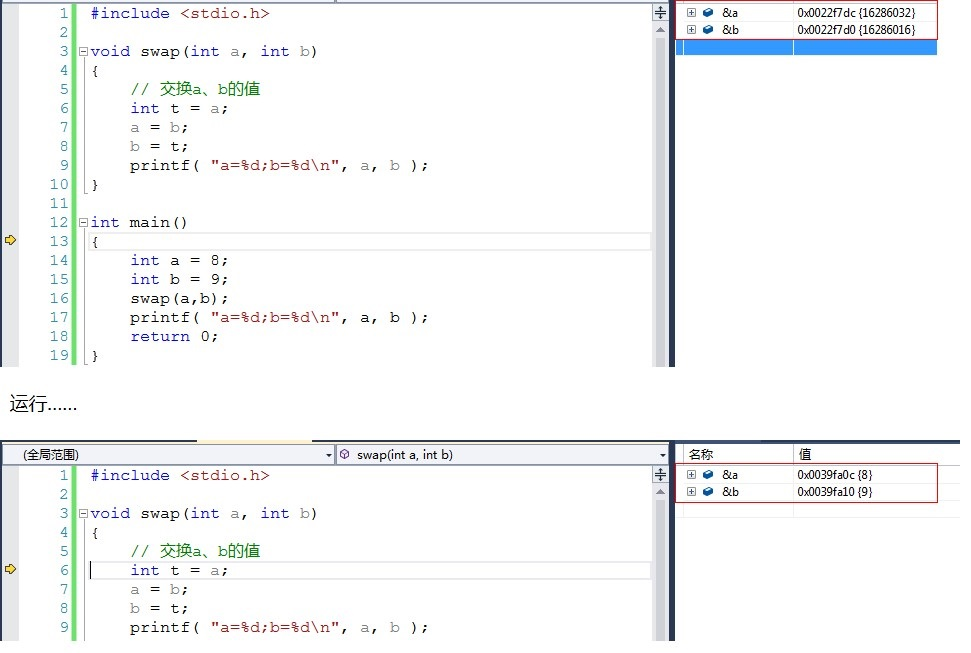
\includegraphics[scale=.6]{../src/swap_01.jpg}
\caption{地址变了}
\label{fig:swap_01}
\end{figure}

这是通过调试的方法,运行时获取到了变量a和变量b的地址,可以看到,从主函数开始(上半截),运行到13行时,a的地址为0x0022 f7dc,b的地址为0x0022 f7d0,但是运行到了第六行(下半截),此时,a的地址是0x0039 fa0c,b的地址变成了0x0022 fa10。 诶,为什么运行运行,运行得把变量地址都改变了?不是的,请看下图:

\begin{figure}[bpht]
\centering
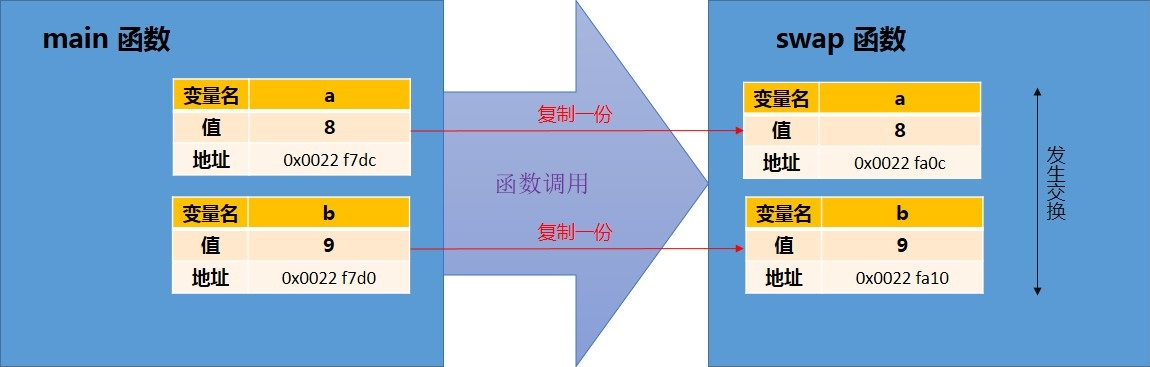
\includegraphics[scale=.5]{../src/swap_02.jpg}
\caption{如此传递}
\label{fig:swap_02}
\end{figure}

看到这,您或许已经想到了,main函数在调用swap函数的时候,是将自己a,b的值分别复制一份给swap函数中的a和b,虽然在main函数中和swap函数中,两个变量名称都叫a和b,但是两个变量所属的函数不同,地址空间也不同,所以,把swap中的a 和b做了交换,跟main函数的a和b就没关系了。就好比我叫LazyCat,您也叫LazyCat,我这有份复习试卷,我把这份试卷复印一份给您,然而您在我给的这份试卷上乱写乱画,但是我的试卷上是不可能出现您的笔迹的。也就是说C语言的传值,永远是传过去一份复制品。

\subsubsection{指针传递}

传递地址也一样,也是传递复制品。先看如下代码:
\begin{lstlisting}
#include <stdio.h>

void swap(int *a, int *b)
{
	// 交换a、b的值
	int t = *a;
	*a = *b;
	*b = t;
	printf( "a=%d;b=%d\n", a, b );
}

int main()
{
	int a = 8;
	int b = 9;
	swap(&a,&b);
	printf( "a=%d;b=%d\n", a, b );
	return 0;
}
\end{lstlisting}

运行结果如下:
\begin{lstlisting}
a=9;b=8
a=9;b=8
请按任意键继续. . .
\end{lstlisting}

这次确实发生了交换,而且是main函数的a、b发生了交换,请看下图:

\begin{figure}[bpht]
\centering
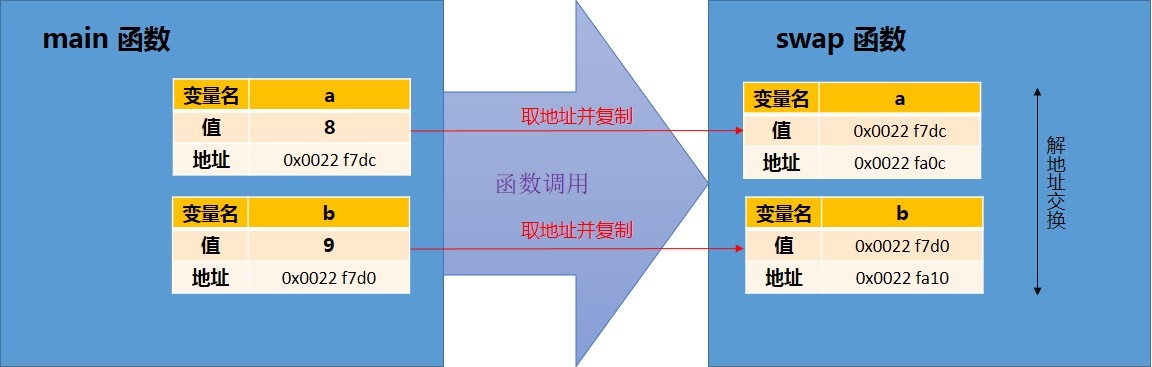
\includegraphics[scale=.5]{../src/swap_03.jpg}
\caption{指针传递}
\label{fig:swap_03}
\end{figure}

从这张图可以看到,swap中的a和b是指针,他们的值分别装了main函数中a和b这两个变量的首地址,当然,swap中的a和b这两个指针同时也拥有自己的地址。在这段代码的6、7、8 行,看到*a,编译器就知道,要从a 装的首地址去找那个值,然后找到地址为0x0022 f7dc这个地方,然后看类型,a是指向整型的,所以从那个地址刨4个字节,然后做相应的处理,*b也一样,所以,main函数的中的a和b 发生了交换。

有个细节希望大家注意,在代码的16行,对应于图中的两处“取地址并赋值”,这其实不是一步操作得到的。第16行的代码应该是下面几行代码合在一起的作用:
\begin{lstlisting}
int *pa = a;
int *pb = b;
swap( pa, pb);
\end{lstlisting}

也就是说,在计算机实现的时候,main函数会另外开辟两块32位的空间\footnote{一般是会开两个寄存器},存放了a和b的地址,调用swap的时候,把pa和pb的值复制一份传过去。所以说C语言中只有传值,传指针也好,传地址也好,都是一样,把值复制一份再传过去。

\subsection{C++引用}
传递引用,这个是C语言没有,C++拥有,有些高级语言如Java,就没有指针,只有引用。在写代码的时候,也同样要注意{\color{red} 扩展名为.cpp而非.c},先看如下代码:
\begin{lstlisting}
#include <stdio.h>

void swap(int &c, int &d)
{
	// 交换 c 、 d 的值
	int t = c;
	c = d;
	d = t;
	printf( "a=%d;b=%d\n", a, b );
}

int main()
{
	int a = 8;
	int b = 9;
	swap(a,b);
	printf( "a=%d;b=%d\n", a, b );
	return 0;
}
\end{lstlisting}

运行结果如下:
\begin{lstlisting}
a=9;b=8
a=9;b=8
请按任意键继续. . .
\end{lstlisting}

首先,请注意这份代码的写法,第三行,注意a和b前面的\&符号,第16行,传递的时候,不用再取地址了。然后看下面这张图:

\begin{figure}[bpht]
\centering
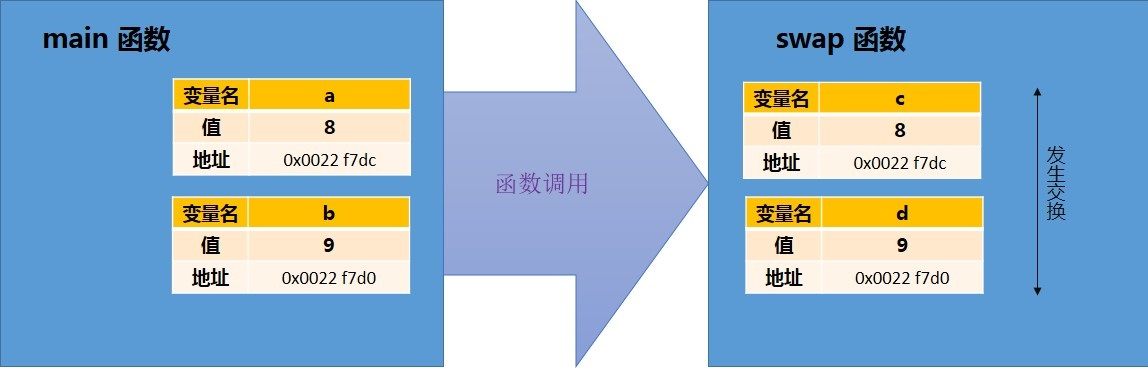
\includegraphics[scale=.5]{../src/swap_04.jpg}
\caption{引用传递}
\label{fig:swap_04}
\end{figure}

可见,swap函数中的c和d与main函数的a和b的地址空间完全相同,所以交换了swap函数中c和d,main函数中的a和b值也是交换了的。这种方式叫做传引用,在swap函数中的c和d相当于给main函数中的a 和b分别取了个别名,就好比您的孩子称呼您为爸爸或者妈妈,而您的父母称呼您为儿子或者女儿,虽然称呼不同,不管是哪种叫法,但是称呼的都是同一个人。

\newpage
\section{新手FAQ}

\subsection{弄清楚C/C++/VC/VS/GCC}
首先,弄清楚C或者C++是一门编程语言,不是一个什么软件,写C语言,可以写在纸上,也可以用Windows自带的记事本写。而VC是Visual C++的简称,是微软公司(Microsoft)针对C语言和C++语言做出来的集成开发环境\footnote{在文首页介绍的时候,那有个脚注,希望您再看看};VS是Visual Studio的简称,是微软的一整套巨型的集成开发环境,不仅支持C/C++语言的,还支持C\#、Visual Basic 等等。GCC是GNU的编译器系列,主要是Linux操作系统下用的。\textbf{语言和开发工具不是等价的,希望大家不要弄混}。

\subsection{VC 6.0 真的不适合新手}
我相信大多数新手在学C语言或者C++语言,尤其是在中国,新手大多入门的时候都是在 Visual C++ 6.0 中写C语言。这款软件是微软公司在1998年发布的,所以它完全不支持后来的C99标准\footnote{其实后续版本的VS中的C编译器也不支持C99标准,除了C99新增的long long关键字以外。VS2013开始支持大部分C99标准。},也不完全支持C++98标准,先看如下几个对比:

\begin{itemize}
\item 64位整型对比:
	$$\begin{tabular}{lll}
	\hline
		& C99标准 & VC 6.0 \\
	\hline
	变量类型 & long long & \_\_int64 \\
	输入输出格式 & \%lld & \%I64d \\
	\hline
	\end{tabular}$$
\item C++语言对for循环作用域范围的问题:

\begin{lstlisting}
for( int i = 1; i < 10; i++ )
{	
	// ...
}
for( int i = 1; i < 10; i++ )
{	
	// ...
}
\end{lstlisting}
首先声明,这种写法在C语言中是错的,但是在C++ 98标准(还包括后来的03,11标准)中是正确的。for中定义的int i变量有仅在for循环内有效。然而VC6.0用的却是C++98之前的 Pre-Standard C++ 语法\footnote{Pre-Standard C++,即国际标准化组织(ISO)在制定C++标准之前的一套通用的C++规范,即C++之父Bjarne Stroustrup写的《The C++ Programming Language (First Edition)》一书中规定的C++语法。},因此,VC6.0会这样认为:
\begin{lstlisting}
int i;
for( i = 1; i < 10; i++ )
{	
	// balabala...
}
int i; // multiple initialization (多重定义)
for( i = 1; i < 10; i++ )
{	
	// HelloKitty
}
\end{lstlisting}
注意第4行和第6行,VC6.0这种理解方法,就是您是编译器,我想也会报错的吧?!

\end{itemize}

总而言之,VC 6.0对C或C++标准支持很烂,可能会误导同学们对标准C或C++的概念,甚是不好。而且有个严重的假死BUG,即有时不管写什么都无法编译执行,编译图标都是灰的。在Windows上,强烈推荐大家使用Visual Studio 2012\footnote{此软件要求在Windows 7上运行。如果您是Windows XP,可以使用Visual Studio 2010,也是不错的。}。VS 2012对新手非常友好,在写代码的时候,只要有编译错误,会立即在你的代码下面画上一条红色的下划线,{\color{red}{\uwave{\color{black}{就}}}}{\color{red}{\uwave{\color{black}{像}}}}{\color{red}{\uwave{\color{black}{这}}}}{\color{red}{\uwave{\color{black}{样}}}},不用等到编译的时候再报错,然后一个个修改。至少VS.NET 2002以上的版本,都支持long long,这点是非常好的!而最推荐大家使用的是GNU的那套工具,但是要求在Linux操作系统的环境中,在此不详细解释。

\subsection{什么是工程}
许多人在Windows中初学C语言,用的是VC/VS之类的\kw{集成开发环境(IDE)}。当我们在里面写代码之前要做什么?——先创建\kw{工程(project,又译作项目)},然后再在这个项目中创建源文件,才开始写代码。那么工程/项目是干什么用的?

试想想,如果没有IDE,那么你应该怎么编译你的源文件?那就是在\kw{命令行}\footnote{例如Windows上的“命令提示符”(cmd)和Linux上的shell。}中键入相应的编译命令,生成目标文件,然后再键入链接命令,生成可执行文件(参见第\pageref{fig:cmpsys}页的图 \ref{fig:cmpsys})。那么我们怎么样才能不打这些编译链接参数呢?那就是预先把编译参数告诉计算机,让它每次按这个流程来编译链接。于是一种方法产生了,这就是工业化生产软件至今常用的技术——Makefile,它是一个文件,编译链接的参数都写在里面。那么如何更傻瓜化一点把Makefile的技术的集成到IDE 中呢?这就是\kw{工程文件/项目文件(project file)}。其实,工程文件/项目文件就是Makefile的一个变种\footnote{这么说其实也不准确,但初学者就先这么理解吧。},只不过它的语法非常地模式化,这样更有利于IDE的解析。如果不建立工程,就单单打开了c或cpp文件,IDE怎么知道您的编译要求是什么呢?

第二个问题是注意我们建立工程的目录,我们建立工程目录时,在弹出来的向导对话框中有个目录,VS2012如下图所示,我们再新建的文件一般就是在这个目录下可以找到,所以不要每次都新建一个项目,这样既浪费了磁盘空间,也不利于查找。我个人推荐的做法就是每次新建一个文件加入该目录,老的文件就全部注释掉,注释很简单,一对/* */就可以搞定了,VS2012还有一对快捷键,先选中代码,一般全选可以按Ctrl+A,然后是注释,先按Ctrl+K,再按Ctrl+C,就注释了,如果要取消注释,可以先选中代码,先按Ctrl+K,再按Ctrl+U。如果你按下Ctrl+K,又不想注释,可以按下Esc取消掉,一般在VS的状态栏的左下角都会有提示的。

\begin{figure}[bpht]
\centering
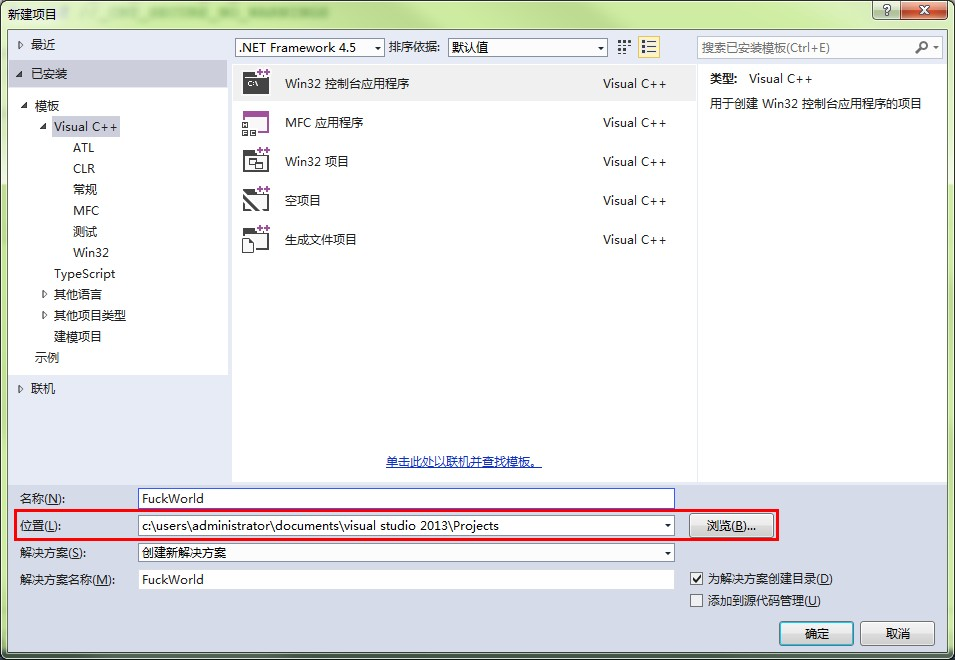
\includegraphics[scale=.5]{../src/projectpath.jpg}
\caption{工程路径}
\label{fig:projectPath}
\end{figure}

\subsection{代码风格}
说起代码风格,这个各种奇葩的风格都有,只要看上去一致、美观都行,以下列出了ANSI 风格和K\&R风格,主要区别在与大括号,各有所长,不影响正常阅读,个人认为风格之争没必要的,您可以随意选择。

\begin{lstlisting}
// ANSI 风格
#include <stdio.h>

int main(void)
{ // 注意这个括号写在函数头的下一行
	int a = 5;
	while( a < 100 )
	{
		printf( "%d\n", a );
		a += 10;
	}
	return 0;
}

// K&R 风格
int main(void) { // 大括号写在函数头的旁边
	int a = 5;
	while( a < 100 ) { // 大括号写在旁边
		printf( "%d\n", a );
		a += 10;
	}
	return 0;
}
\end{lstlisting}

在此,我还想强调一个问题,是关于\kw{空格(spcace)}和\kw{制表符(Tab)}这两个\kw{缩进(indent)}符,一般来说,Windows下默认一个Tab是4个空格字符的宽度,Linux下默认是8个,注意在上面的代码,main函数下的int a = 5;这条语句,以及while 下printf语句,前面空白部分我都是由Tab构成,int前面一个Tab,printf前面2个Tab,我并没有用空格,有两个原因,最明显的原因是因为空格字符要打4个或8 个,难打,而且退格的时候,Tab只要按一下退格就OK 了,空格就要退4次或者8次;更重要的原因是有很多其他语言(比如python)的代码不是以大括号分段,在C语言我们写if、while之类的,后面接一对大括号\{ \},里面的东西都归if、while管,但是那些语言是依靠Tab来区分哪些代码属于这个分支的,哪些代码属于那个循环管的,所以区分Tab和空格是很严格的,不像C代码中这样自由。所以给您一个建议,养成一个良好的使用Tab的习惯。

\subsection{i++和++i}

先看如下代码:
\begin{lstlisting}
#include <stdio.h>

int main(void)
{
	int i = 0;
	printf("%d,%d\n", i++, i++);
	i = 0;
	printf("%d,%d\n", ++i, ++i);
	return 0;
}
\end{lstlisting}

我不想问您输出结果,因为我不想被人骂脑残!这个代码编译后执行的结果,完全取决于编译器。不同的编译器,在编译的时候,具体在哪一步把i给自加1,只有编译器知道。C 标准对此定义为\kw{未定义行为(undefined behavior)}。 这种行为,编译器想怎么加就怎么加,想在什么时候加就在什么时候加,所以编译的结果不同,即使是相同的编译器,不同的编译参数编译结果也不同。

C标准(包括C89标准、C99标准、C11标准)规定,函数实参的运算顺序是没有先后的,诸如f(x)+g(x)的f函数和g函数的调用顺序也是没有先后的,可以从左往右,也可以从右往左,甚至可以先中间后两边,还可以随机运算,或者多线程并发运算,或者多核并行运算。因此\verb|printf("%d,%d\n", i++, i++);|的两个i++的先后顺序是不确定的,这种未定义的SB代码还有\verb|b = (a++)+(a++);| 等等。

所以在写代码时,使用$++/--$这些符号的时候,每条语句仅使用一次,才是最好的。

\subsection{去掉大括号}
我们在学C或C++时,分支,循环,大体都是如下格式:
\begin{lstlisting}
if()
{
	a++;
}
else
{
	a--;
}

while()
{
	a++;
}
for(;;)
{
	c++;
}
\end{lstlisting}

这里我并没有写小括号中的表达式,只要满足条件,就执行这对花括号里面的内容,但是注意到,这个花括号里面只有一条语句,因此我们可以简写为:
\begin{lstlisting}
if()
	a++;
else
	a--;

while()
	a++;
for(;;)
	c++;
\end{lstlisting}

也就是说,花括号可以去掉。这种情况只发生在分支体或循环体仅仅只有一条语句的时候,而且请注意,else只能跟最近的if或者elseif配套,如:
\begin{lstlisting}
if()
	for()
		if()
			a++;
else()
	c++;
\end{lstlisting}

看上去这个else与第一行的else匹配,实际上跟第三行的对应。因为C或C++这种依靠花括号来划分归属关系的,并不是像python那种根据缩进来划分的。要跟第一行对应,那就得在第一行后面加个大括号,在第四行最后加上反大括号。最后再说明下,\textbf{这种情况不能推广到函数,也就是说函数体内哪怕只有一句话,也不能省略大括号!}

\subsection{您写对过主函数吗?}

先看看《ISO/IEC 9899:1999》(俗称C99标准)中的5.1.2.2.1条的规定。

\begin{figure}[bphtH]
\centering
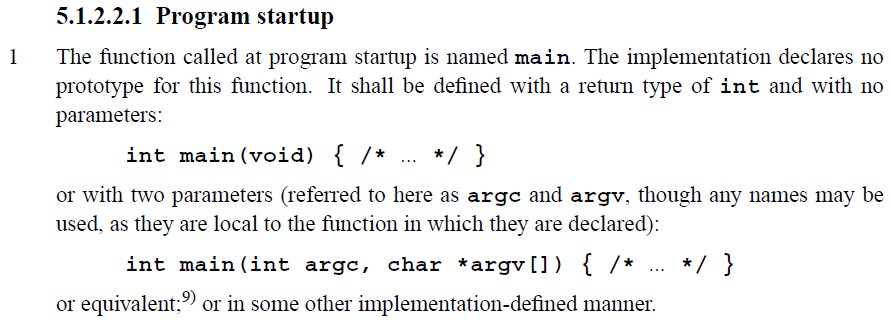
\includegraphics[scale=.5]{../src/C99main.jpg}
\caption{C99标准对main函数的规定}
\label{fig:C99main}
\end{figure}

这里说的很清楚,只有\verb|int main(void)|和\verb|int main(int argc, char *argv[])|是C99标准明文规定的,其它原型的都是编译器扩展。常见的C编译器常见的非标准扩展中,main函数还有第三个参数char *env,用于传入一些操作系统的环境变量,所以在某些时候可能看到int main(int argc, char *argv[], char *envp[])和int main(int argc, char *argv[], char *envp[], char *apple[]),但这也是非标准的,所以不建议使用\footnote{如果到了某天您成了大神,一定要传环境变量,记得我曾在此写下的,请使用getenv()函数,当然,也请加上头文件<stdlib.h>。}。

我看到很多新手,在写主函数的时候,写成void main()的形式,这种形式非常离谱,也非常不合规定,尤其到了C++中:

《ISO/IEC 14882:1998》(俗称C++98标准)中的3.6.1条规定:

\begin{figure}[H]
\centering
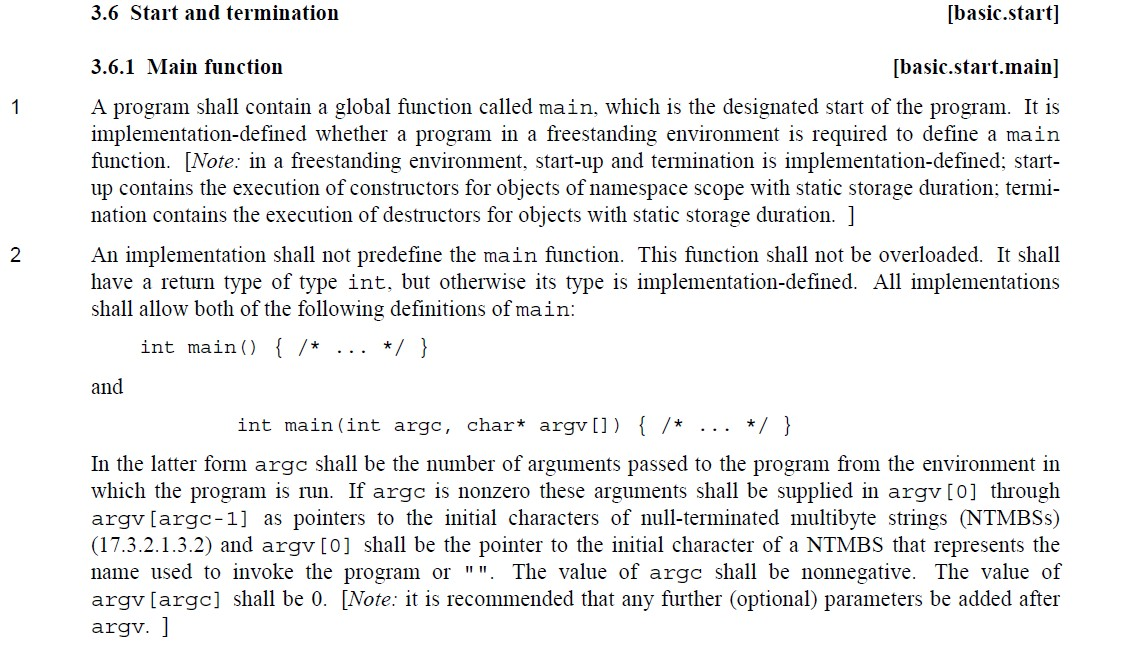
\includegraphics[scale=.5]{../src/cpp98main.jpg}
\caption{C++98标准对main函数的规定}
\label{fig:cpp98main}
\end{figure}

《ISO/IEC 14882:2011》(俗称C++11标准)中的3.6.1条规定:

\begin{figure}[H]
\centering
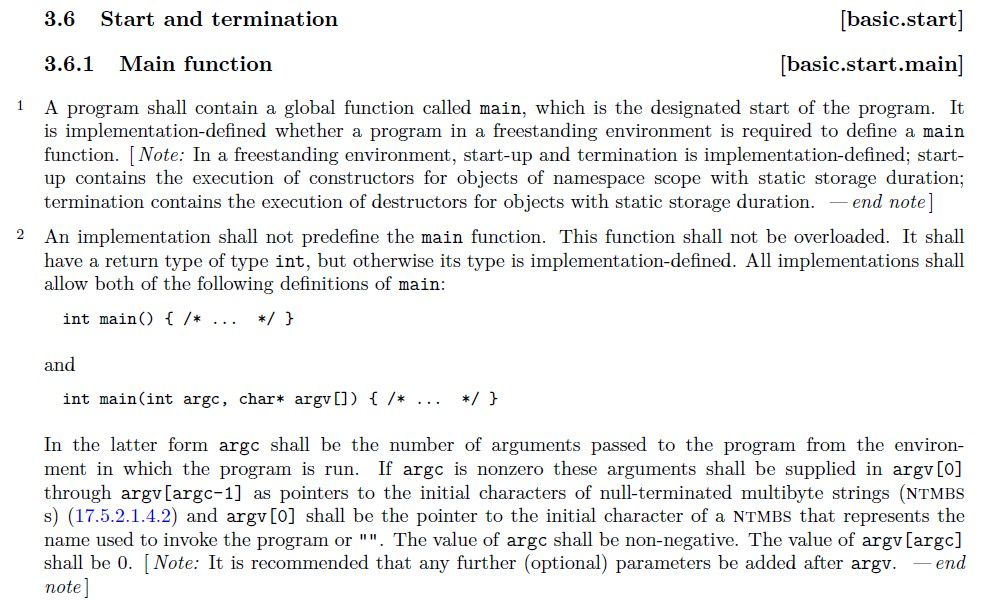
\includegraphics[scale=.45]{../src/cpp11main.jpg}
\caption{C++11标准对main函数的规定}
\label{fig:cpp11main}
\end{figure}

说得很清楚,C++98标准和C++11标准中,main函数的声明有两种,即\verb|int main()|和\verb|int main(int argc, char* argv[])|,而且还比C语言标准中说的更严格,明文说出了It shall have a return type of type int (它必须有一个int类型的返回值)。也就意味着,C++语言中绝对禁止void main(),连作为非标准扩展的权力都没有(C标准好歹还允许void main作为非标准扩展)。因此,C++的要求更严格,void main 直接编译错误。凡是能够编译通过的,如果发出警告信息还好,连警告都没有的,那绝对是不遵守C++标准的编译器。

在此我并不想阐述主函数的参数、返回值的具体作用,但是希望大家要养成一个遵守使用标准C或标准C++的习惯,即使以前写的是void main,也希望您能纠正过来,严谨的态度是很重要的。

\subsection{C标准和C++标准}

\begin{itemize}
\item 《ANSI X3.159-1989》,1989年发布,简称C89标准或ANSI C标准。后来,在1990年,国际标准化组织ISO通过了C89标准,命名为《ISO/IEC 9899:1990》,简称C90标准。所以C89标准与C90标准完全等同,不过业界更常使用“C89标准”这个术语,很少出现“C90标准”这个术语。

目前所有C编译器都支持C89标准。
\item 《ISO/IEC 9899:1999》,1999年发布,简称 ISO C 99 标准。

目前gcc、clang、Intel C++、Borland C++等各大主流C编译器支持C99标准,但微软Visual Studio 2012的除了long long以外,都不支持。Visual Studio.NET 2002开始支持long long,Visual C++ 6.0不支持。Visual Studio 2013开始支持绝大部分的C99标准。
\item 《ISO/IEC 9899:2011》,2011年发布,简称 ISO C 11 标准。

C11标准的支持情况不佳,目前只有最新版的gcc和clang支持C11标准。

\item 1985年,Bjarne Stroustrup写了一本书,名叫《The C++ Programming Language》。这本书就是C++语言的第一部\kw{事实标准(standard de facto)}。

在此之后,国际标准化组织(ISO)发布了三套C++语言的正式标准:
\item 《ISO/IEC 14882:1998》,1998年发布,简称 ISO C++ 98 标准,又名 ANSI C++ 标准。

Intel C++、g++、clang++、Borland C++等等,都支持C++98标准。微软Visual C++ 6.0部分支持C++98标准,Visual Studio.NET 2002开始完全支持C++98标准。

\item 《ISO/IEC 14882:2003》,1998年发布,简称 ISO C++ 03 标准。

C++03标准是C++98标准的“bug修复版”,与C++98标准几乎没什么区别。所以说支持C++98标准和支持C++03标准的编译器没有什么区别。

\item 《ISO/IEC 14882:2011》,2011年8月12日发布,简称 ISO C++ 11 标准。

g++、clang++等等,都支持C++11标准。Intel C++ 2013 部分支持C++11标准。微软Visual Studio 2010开始部分支持C++11标准\footnote{在C++11标准出来之前,ISO就发布了这套标准的草案,草案名叫C++0x,所以Visual Studio 2010实际上支持的是C++0x 草案。},Visual Studio 2012基本上支持C++11标准,当然Visual Studio 2012对C++11标准的支持的还是有很多bug的\footnote{例如这个bug:\href{http://connect.microsoft.com/VisualStudio/feedback/details/804635/bug-in-lambda-expression-in-visual-studio-2012-update-3}{Visual Studio 2012 在 C++ 11 的 Lambda 表达式的支持上的bug}。不知道您看这篇文章时是否修复了}。

\item 《ISO/IEC 14882:2014》,2014年8月18日发布,简称 ISO C++ 14 标准。

C++14标准只是C++11标准的一些功能性的补充,对C++11标准的一些过于严格的限制进行适当的放松,可以说仅仅一个“微调”,与C++11标准没有太大的区别。

VS2013支持一小部分的C++14标准\footnote{参数资料:\url{http://www.infoq.com/news/2013/11/VC13_CTP1} }。clang++ 3.4已经完全实现了全部的C++14标准\footnote{参考资料: \url{http://clang.llvm.org/cxx_status.html} }。

\end{itemize}

最后说下如何获得C或者C++标准的文档,请登录\url{http://www.ansi.org/}联机购买一本电子副本(PDF)。呃,先说明,要花money的,您懂的。

\subsection{函数声明}
先看如下代码

\begin{lstlisting}
#include <stdio.h>

int main(void)
{
	fun(3);
	return 0;
}

void fun(int x)
{
	x++;
	printf("Are you OK?\n");
}
\end{lstlisting}

这段华丽丽的函数调用代码在编译的时候会报错,什么错?无法找到fun函数。但是我们这么写:

\begin{lstlisting}
#include <stdio.h>

void fun(int x)
{
	x++;
	printf("Are you OK?\n");
}

int main(void)
{
	fun(3);
	return 0;
}
\end{lstlisting}

就是说我把fun函数先写在前面,就通过了。这是什么原因呢?在第一份代码中,我们把fun写在main函数的后面,那么在编译的时候,先编译main函数,此时,还没有编译fun 函数,所以编译器没有关于fun函数的信息,现在又要调用fun 函数,编译器怎么知道fun函数在哪?但是第二份代码中,先编译了fun函数,那么编译器就知道fun函数在哪了,当然,也就可以调用了。

我们在第一份代码的第二行加入如下代码:
\begin{lstlisting}
void fun(int);
\end{lstlisting}

我们加上这一行代码便可以通过,这行代码叫\kw{函数声明(function declaration)},编译在编译主函数之前,看到函数声明,知道有个叫fun的函数,参数为一个int,返回值为void的函数将会出现,而且名字叫fun,在此,编译器会做个记号,知道有这么个东西,然后在编译main函数时,调用fun,编译器就知道,这调用的是前面说过的那个fun,需要的什么参数,返回方式等等,就可以为这个函数做一些调用所需要的准备工作,来迎接fun函数(第一份代码因为不知道fun函数的相关信息,所以没法做准备工作)。然后继续往下面编译,把下面这个fun的实现编译完。最后链接的时候,将声明的fun,与这个fun的实体联系起来,就O 了。

注意看这个函数声明,写形参的时候,我只写了int,并不是int x,这个x可写可不写,但是一般不写,一来告诉main函数类型就够了,二来如果写成了int x,万一下面的fun 函数的参数写成int y,严格一点的链接器,就会认为参数不正确,无法将声明和实现绑定。

\subsection{循环输入}
先看如下代码

\begin{lstlisting}
#include <stdio.h>

int main(void)
{
	int a, b;
	scanf("%d%d", &a, &b);
	printf("%d\n", a+b);
	return 0;
}
\end{lstlisting}

最常见的a+b,但是我们每次执行,输入一个a,一个b然后输出结果,要重新输入两个数的时候,却不得不重新再打开执行,我要输入20组a和b,就要打开20次,这样做非常麻烦,请看下面代码,对比上面代码

\begin{lstlisting}
#include <stdio.h>

int main(void)
{
	int a, b;
	while( scanf("%d%d", &a, &b) != EOF )
			printf("%d\n", a+b);
	return 0;
}
\end{lstlisting}

可以发现我们多了个while循环,scanf是个函数,他有返回值,返回的是输入变量的个数,这里返回值是2,因为有a和b两个变量被输入了。当scanf的返回值不等于EOF的时候,执行循环体,那么这个EOF是什么呢?

EOF,即End of File,中文直译就是文件结束的地方,是个宏,值就是-1。当scanf的返回值为-1的时候\footnote{注意,scanf的返回值不是您输入的值,您输入-1,scanf认为您输入了一个数,返回值至少为1},就代表输入结束了,可能您有点疑问了,这个文件跟我从键盘输入有什么关系啊?在操作系统设计理念上,有句著名的话,叫 Everything is a file!”,这个文件的含义,跟我们惯性思维下硬盘上的文件是有区别的,在此并不解释其中奥义,但是请您记住,\textbf{对于应用程序来说,所有设备,诸如键盘、鼠标、显示器、打印机、音箱、硬盘、网卡等等都是文件},敲了某个键,对于应用程序来说,就是从键盘这个文件中读取到了一个字符,输出一个字符,就是往显示器这个文件中写入一个字符。而且请注意,一般我们把\kw{标准输入文件(standard in file)}对应的就是键盘文件,\kw{标准输出文件(standard out file)}对应的便是显示器文件\footnote{这句话不完全正确,但是大家现在暂时可以先这么理解。如果您非常了解操作系统,您就会知道其中细微的分歧了。}。

所以当我们scanf输入时,没有输入到键盘文件结尾,就会一直输入下去。但是您可能会问,我早就没按键盘了,难道不就是输入到结尾了吗?不是的,没有按键盘并不等于输入到结尾,但是如果您在Windows 命令提示符中按下了Ctrl+Z\footnote{Linux 中用的是Ctrl+D},再按回车,这就是键盘文件的结束了;如果在控制台程序下按下了Ctrl+C,那么就是强行退出程序,注意这跟按Ctrl+Z还是有区别的。

还有个有意思的问题,叫做重定向输入输出,我并不打算写了。有兴趣的可以去查阅相关资料,重定向输入输出用的最广的,莫过于打表了,哈哈哈哈~

\subsection{补码计算规则}
很多人认为补码就是二进制原码取反再加上1,这是根本就是错误的!原码取反加1只不过是求补码的一种快捷的计算方法罢了,他并不是补码的本质,而且有些数的补码是无法用这种快捷方法来计算的。

举个例子吧,一个二进制数,只有3位,$a_2a_1a_0$,而且$a_2$还是符号位,现在用这个3位的二进制数,以原码的方式表示十进制的-4。首先,因为是负数,所以符号位要为1,即$a_2$为1,然后,剩下的这个4,只有两位2进制如何表示这个4呢?两位二进制,最大的不过$(11)_2$,化成10进制也只有3,如何表示4呢?没错,在原码中3位二进制是没办法表示这个-4的,但是在补码中可以表示-4,而且补码形式就是$100$。

经常看到某些书或某些人说什么什么正数补码等于原码,负数原码取反加一变补码,补码取反加一变原码,那么现在请您把$100$这个补码先取反得到$011$,再加1,得到所谓的原码,可以看到,原码也是$100$,这个原码是什么意思?符号位为1,表示负数,后面的全是0,这就是传说中的负零?负零跟零是几个意思?

其实补码这个翻译方式我个人感觉就不对,应该翻译成带权码之类的。一个二进制数,如果没有符号位,我们称之为无符数,例如一个8位无符号的二进制数$1010\ 0101$,化成10 进制,就是:
$$1\times 2^7 + 0\times 2^6 + 1\times 2^5 + 0\times 2^4 + 0\times 2^3 + 1\times 2^2 + 0\times 2^1  + 1\times 2^0 = 128+32+4+1 = 165$$
请看如下式子:
$$\textcolor[rgb]{1.0,.0,.0}{(-1)\times 2^7} + 0\times 2^6 + 1\times 2^5 + 0\times 2^4 + 0\times 2^3 + 1\times 2^2 + 0\times 2^1  + 1\times 2^0 = -128+32+4+1 = -89$$

可以观察到两个式子,在最高位,第一个是按正$1\times 2^7$计算,第二个是按$-1\times 2^7$计算。十进制164和-89都是用$1010\ 0101$这个二进制数表示,当$1010\ 0101$ 表示无符号数时,按照第一种方式计算它的十进制值,当$1010\ 0101$ 表示有符号时,按第二种方法计算它表示的十进制的值,这种计算方法,正是补码最原始的计算方法。

计算机规定最高位为符号位,那好,现在我自己规定,最低位为符号位,那么$1010\ 0101$按补码的形式化成十进制成了:
$$1\times 2^7 + 0\times 2^6 + 1\times 2^5 + 0\times 2^4 + 0\times 2^3 + 1\times 2^2 + 0\times 2^1  + \textcolor[rgb]{1.0,.0,.0}{(-1)\times 2^0} = 128+32+4-1 = 163$$

所以根据符号进行展开计算相加才是补码的最根本的计算方法,也是补码的实质所在。回到计算机中,按计算机中的规定,最高位为符号位,如果现在是这样一个有符号的二进制数$0010\ 0101$,化成十进制为:
$$\textcolor[rgb]{1.0,.0,.0}{(-0)\times 2^7} + 0\times 2^6 + 1\times 2^5 + 0\times 2^4 + 0\times 2^3 + 1\times 2^2 + 0\times 2^1  + 1\times 2^0 = 32+4+1 = 37$$
注意那个红色部分,我故意这么写的。-0就是0,0乘以任何数得0,那这样写跟我们所谓的原码$0010\ 0101$代表的值还有区别吗?这也正是所谓的正数的原码等于补码的原因了。如果是负数,上面不是有个-89吗?89 的二进制是$0101\ 1011$,取反$1010\ 0100$,再加上1,得到$1010\ 0101$,正好跟上面的补码-89相同,也就说在最高位为符号位时,原补码取反加一这种计算方法成立,但是像我那样,规定最低位为符号位,那还成立吗?

而且这种取反加一的计算方法,无法解释最高位为1,其余位为0的二进制补码数,就像本小节开始提到的100三位有符号二进制数补码可以表示-4,但是没有对应的原码,\textbf{所以取反加一只是补码与原码相互转化的一种机制而已,并不是补码的真正意义}!

\subsection{溢出问题}
\begin{lstlisting}
#include <stdio.h>

int main(void)
{
	int a, b;
	while( scanf("%d%d", &a, &b) != EOF )
			printf("%d\n", a+b);
	return 0;
}
\end{lstlisting}

相信这个程序大家都不陌生,输入3和5,输出8,输入2和5,输出7,没问题,但是,我们现在输入2147483647和1,看看结果是多少?如果您没测试,直接回答是2147483648,那么您错的一塌糊涂!

答案是负数,是-2147483648!理论如下:

int为整型,用4个字节表示,每个字节8位,共32位,而且最高位为符号位,正数时,符号位为0,所以二进制最大值为:
$$(0111\ 1111\ 1111\ 1111\ 1111\ 1111\ 1111\ 1111)_2$$
按照补码规则化成10进制就是:
$$1\times 2^0 + 1\times 2^1 + 1\times 2^2 +\dots +1\times 2^{30} = \sum^{30}_{i=0}2^{i} = 2^{31}-1 = 2147483647$$

一旦超过这个数,就像上面的加法一样,现在把这个数加1,那么二进制表示就成了:
$$(1000\ 0000\ 0000\ 0000\ 0000\ 0000\ 0000\ 0000)$$
按照补码规则化成10进制:
$$0\times 2^0 + 0\times 2^1 + 0\times 2^2 +\dots +0\times 2^{30} +(-1)\times 2^{31} = (-1)\times 2^{31} = -2147483648$$

这还不能算典型的溢出,顶多就是溢到了最高的符号位,但是我要是乘法了?比如$2147483647\times 3$

\begin{tabular}{cr}
 & $(0111\ 1111\ 1111\ 1111\ 1111\ 1111\ 1111\ 1111)_2$ \\
$\times $ & $(11)_2$ \\
\hline
 & $(0111\ 1111\ 1111\ 1111\ 1111\ 1111\ 1111\ 1111)_2$ \\
+ & $(0\ 1111\ 1111\ 1111\ 1111\ 1111\ 1111\ 1111\ 1110)_2$ \\
\hline
& $(1\ 0111\ 1111\ 1111\ 1111\ 1111\ 1111\ 1111\ 1101)_2$
\end{tabular}

很明显,最后的结果,超过了32位,我们称之为\kw{溢出(overflow)}。

怎么解决呢?一个很合理的方法是使用更多位来表示这个整数,在C99标准和C++11标准中规定可以用long long 表示,输入输出格式为"\%lld"\footnote{微软VC6.0 用\_\_int64,注意是双下划线,输入输出用"\%I64d"。自VS.NET2002起,二者都支持。},那么代码可以写成:

\begin{lstlisting}
#include <stdio.h>

int main(void)
{
	long long a, b;
	while( scanf("%lld%lld\n", &a, &b) != EOF )
			printf("%lld\n", a+b);
	return 0;
}
\end{lstlisting}

这时,可以试试输入2147483647和1,结果就是2147483648。但是long long是64位的有符号整数,也就说它表示的值也有上限。通过以上的推导,可以得出long long的上限是$2^{63} -1$,那么更大的数呢?没办法了,只能开数组去模拟,如果您会Java的话,BigInteger简直太妙了~

还有个溢出问题是比较让人郁闷的。比如a、b、c、d四个都是int型32位整数,现在已知a、b和c,且已知$d = a\times b\div c$(假设满足整除关系),虽然估计最终结果d不会超过32位,但是$a\times b$这个中间结果可能溢出,这样就会导致最终结果发生溢出,最简单粗暴的方法就是交换计算顺序,即改成 $d = a\div c\times b$ 即可.

\subsection{格式化输出}
这个问题主要是针对如何输出只有两位小数的浮点数,如何控制字符宽度,右对齐、左对齐之类的,在此我并不想详细说,给出大家一个网址,相信您一看就懂:

\url{http://www.cplusplus.com/reference/cstdio/printf/}

\subsection{OJ常见反馈信息}

\noindent\begin{longtable}{p{\dimexpr.3\textwidth-1\tabcolsep-0.8pt}
                   p{\dimexpr.7\textwidth-1\tabcolsep-0.4pt}}
\hline
名称 & 解释 \\
\hline
Queuing & 排队,提交太多了,排队等候 \\
Pending & 阻挡,效果同上 \\
Compiling & 您的代码正在被编译 \\
Running & 您的代码正在运行 \\
Judging & 正在判断您的代码是否正确 \\
Accepted (AC) & 通过,即答案正确 \\
Present \seqsplit{Accepted} (PA) & 目前通过,比赛结束后会用更多数据来检测是否完全通过 \\
Wrong Answer (WA) & 答案错误 \\
Presentation Error(PE) & 格式错误,即计算结果对的,但是输出格式不对 \\
Runtime Error (RE) & 运行时错误,程序非法操作 \\
Segment Fault (SF) & 段错误 \\
Time Limit \seqsplit{Exceeded} (TLE) & 程序运行时间超出题目规定时间 \\
Memory Limit \seqsplit{Exceeded} (MLE) & 程序运行使用的内存超出规定限制 \\
Output Limit \seqsplit{Exceeded} (OLE) & 程序输出内容太多,超过了这个题目的输出限制 \\
Compilation \seqsplit{Error} (CE) & 编译错误,有语法错误或者选错编译选项 \\
System Error (SE) & 系统错误,OJ挂了 \\
Out Of Contest Time & 超出比赛时间,也就说比赛结束再提交无效 \\
\hline\\
\end{longtable}


特别说明一下,那个Runtime Error(RE)和Segment Fault(SF)大多是程序的指针乱飞、数组越界问题,或者是爆栈了,浮点数上下溢出,除数为0等等,此外RE出现还有可能调用了OJ所规定的不能调用的\kw{系统调用(system call)},比如:system("shutdown -s -t 0")。

\newpage
\section{其他}
\subsection{推荐书籍}
计算机类书籍很多,以下书籍仅仅只是推荐给初学者,尤其是学C或C++开始的初学者。如果您还学到了其他知识,诸如数据库、Java等等,那么抱歉,我在此并没有写出相关书籍。也许您还注意到,我推荐的都是外国的是书籍,您可以看对应的中文版的。中文的书籍有好的,比如侯捷的《深入浅出MFC》,但那不是给初学者的了。如果您想说谭浩强先生的书不错,如果您读了我在FAQ那章写到的关于主函数的问题,您或许就明白我为什么不推荐了。

\noindent\begin{tabular}{lll}
\hline
书名&作者(仅列出一位作者) \\
\hline
The C Proguamming Language & Brian W.Kernighan \\
C Primer Plus & Stephen Prata \\
C++ Primer & Stanley B.Lippman \\
C++ Primer Plus & Stephen Prata \\
Professional C++ & Marc Gregoire \\
Thinking in C++ & Bruce Eckel \\
Discrete Mathematics and Its Applications & Kenneth H.Rosen \\
Date Structures and Algorithm Analysis in C & Mark Allen Weiss \\
Computer Systems & Randal E.Bryant \\
Concrete Mathematics & Ronald L.Graham \\
Introduction to Algorithms & Thomas H.Cormen \\
Modern Operating System & Andrew S.Tanenbaum \\
Expert C Programming & Perter Van \\
\hline
\end{tabular}

\subsection{推荐网站}
\begin{tabular}{ll}
\hline
名称 & 网址 \\
\hline
维基百科 & \url{http://en.wikipedia.org/wiki/Main_Page} \\
“栈溢出”IT技术问答网 & \url{http://stackoverflow.com/} \\
百度百科 & \url{http://baike.baidu.com/} \\
C++参考——C++资源网 & \url{http://www.cplusplus.com/} \\
cppreference.com & \url{http://en.cppreference.com/w/} \\
C语言常见问题集 (中文) & \url{http://c-faq-chn.sourceforge.net/} \\
\hline
\end{tabular}

两个百科,维基和百度,通过词条检索关键词了解相关知识,虽然维基可以切成中文,但是我更倾向您阅读维基上面的英文,因为有些词条英文更详细全面。StackOverflow是国外的专门解答IT技术的网站,但是是全英文的。C++编程和reference,从名字上就可以得出,其作用是干什么的。C语言常见问题集网站提供相关链接,您可以下载相关内容查看,比我这里的FAQ写得更全面,更详细。

\subsection{版本说明}
如果您有幸看到本版且是最新版,那么恭喜您,您看到的是第一版。说实话,我并不打算写这个东西,但是有朋友总是问我同样的一些问题,有些只是为了应付二级C语言罢了,有些朋友是学计算机专业的,刚刚入门。但是很突出的一个问题是他们不明白地址这个东西,所以有很多C语言的东西朋友们无法理解,死记都很容易忘。跟朋友们解释一遍又一遍,文字聊天时相同的文字,打了好几十遍了,所以我打算一劳永逸,便写下了这篇文章。原来这篇文章并不打算写长,只想写几页纸罢了,但是一写起来发现要写的东西实在是太多了,而且我已经砍掉了很多东西,这个可以在文章多出写到的“在此不详谈”之类的话。只能说计算机太复杂了。

写这篇文章时间确实有点短,文章中难免出现错误,有时我写的东西,我写的时候是正确的,但是没过多久就是错的,因为计算机发展太快了,我也不知道下一秒会有什么样的翻天覆地的变化。所以如果您看到本文有什么不正确的地方,不吝赐教,请发送邮件\href{mailto:Freagle@yeah.net}{Freagle@yeah.net}联系本人,本人感激不尽。

\subsection{致谢}
首先第一要感谢的是飞哥,虽然他是个节操吞噬狂魔,但是飞哥对本文的校验起到很大的帮助,可以说是本文的主审。说实话,有些内容写出来我自己去读,都觉得狗屁不通,还好飞哥给我做了些调整。而且最后的FAQ有一半是他所写的,我只不过是砍掉了一些,调整了一些,因为飞哥写得太专业,怕新手朋友看不懂。在最后的推荐网站,由于时间关系,我都是拜托飞哥写的。所以在此十分感谢飞哥!

还有不翻墙的好孩子丁丁小朋友,作为我的小学、初中同学,高中和大学校友,学的并不是计算机专业。呃,丁丁小朋友曾向我反应过局部变量的问题,虽然这是个小问题,但是讨论这个问题,就麻烦大了,再三犹豫下,我还是放弃了。

还有小孙子,呃,作为孙神,眼神就是好啊,果断能看出句子成分残缺。不过孙神说没看懂未定义行为,本来是飞哥详细写的,被我怒删了,怕新手朋友看不懂。不过在此可以简单补充一句:未定义行为就是胡作非为,哪怕结果没有任何合理性,哪怕引爆你的电脑,都算在内。

还要感谢其他的朋友,告诉我哪里打错字了,或者哪个词语用错了,甚至是中文语法错误(/ □ \textbackslash)。在此一并表示忠心感谢。

最后,感谢党和国家\footnote{呃,是的}。
%\prinindex									% 输出所有索引
\end{document}
%--------------------------------------------------------------































